\documentclass[a4paper]{book}

\usepackage{geometry}
% make full use of A4 papers
\geometry{margin=1.5cm, vmargin={0pt,1cm}}
\setlength{\topmargin}{-1cm}
\setlength{\paperheight}{29.7cm}
\setlength{\textheight}{25.1cm}

% auto adjust the marginals
\usepackage{marginfix}

\usepackage{amsfonts}
\usepackage{amsmath}
\usepackage{amssymb}
\usepackage{amsthm}
%\usepackage{CJKutf8}   % for Chinese characters
\usepackage{ctex}
\usepackage{enumerate}
\usepackage{graphicx}  % for figures
\usepackage{layout}
\usepackage{multicol}  % multiple columns to reduce number of pages
\usepackage{mathrsfs}  
\usepackage{fancyhdr}
\usepackage{subfigure}
\usepackage{tcolorbox}
\usepackage{tikz-cd}
\usepackage{listings}
\usepackage{xcolor} %代码高亮
\usepackage{braket}
\usepackage{algorithm} 
% \usepackage{algorithmicx}  
% \usepackage{algpseudocode}
\usepackage{algpseudocode}  
\usepackage{amsmath}  

\floatname{algorithm}{算法}  
\renewcommand{\algorithmicrequire}{\textbf{输入:}}  
\renewcommand{\algorithmicensure}{\textbf{输出:}}  
\renewcommand{\algorithmicrequire}{\textbf{Input : }}
\renewcommand{\algorithmicrequire}{\textbf{Precondition : }}
\renewcommand{\algorithmicensure}{\textbf{Output : }}
\renewcommand{\algorithmicensure}{\textbf{Postcondition : }}
%------------------
% common commands %
%------------------
% differentiation
\newcommand{\gen}[1]{\left\langle #1 \right\rangle}
\newcommand{\dif}{\mathrm{d}}
\newcommand{\difPx}[1]{\frac{\partial #1}{\partial x}}
\newcommand{\difPy}[1]{\frac{\partial #1}{\partial y}}
\newcommand{\Dim}{\mathrm{D}}
\newcommand{\avg}[1]{\left\langle #1 \right\rangle}
\newcommand{\sgn}{\mathrm{sgn}}
\newcommand{\Span}{\mathrm{span}}
\newcommand{\dom}{\mathrm{dom}}
\newcommand{\Arity}{\mathrm{arity}}
\newcommand{\Int}{\mathrm{Int}}
\newcommand{\Ext}{\mathrm{Ext}}
\newcommand{\Cl}{\mathrm{Cl}}
\newcommand{\Fr}{\mathrm{Fr}}
% group is generated by
\newcommand{\grb}[1]{\left\langle #1 \right\rangle}
% rank
\newcommand{\rank}{\mathrm{rank}}
\newcommand{\Iden}{\mathrm{Id}}

% this environment is for solutions of examples and exercises
\newenvironment{solution}%
{\noindent\textbf{Solution.}}%
{\qedhere}
% the following command is for disabling environments
%  so that their contents do not show up in the pdf.
\makeatletter
\newcommand{\voidenvironment}[1]{%
\expandafter\providecommand\csname env@#1@save@env\endcsname{}%
\expandafter\providecommand\csname env@#1@process\endcsname{}%
\@ifundefined{#1}{}{\RenewEnviron{#1}{}}%
}
\makeatother

%---------------------------------------------
% commands specifically for complex analysis %
%---------------------------------------------
% complex conjugate
\newcommand{\ccg}[1]{\overline{#1}}
% the imaginary unit
\newcommand{\ii}{\mathbf{i}}
%\newcommand{\ii}{\boldsymbol{i}}
% the real part
\newcommand{\Rez}{\mathrm{Re}\,}
% the imaginary part
\newcommand{\Imz}{\mathrm{Im}\,}
% punctured complex plane
\newcommand{\pcp}{\mathbb{C}^{\bullet}}
% the principle branch of the logarithm
\newcommand{\Log}{\mathrm{Log}}
% the principle value of a nonzero complex number
\newcommand{\Arg}{\mathrm{Arg}}
\newcommand{\Null}{\mathrm{null}}
\newcommand{\Range}{\mathrm{range}}
\newcommand{\Ker}{\mathrm{ker}}
\newcommand{\Iso}{\mathrm{Iso}}
\newcommand{\Aut}{\mathrm{Aut}}
\newcommand{\ord}{\mathrm{ord}}
\newcommand{\Res}{\mathrm{Res}}
%\newcommand{\GL2R}{\mathrm{GL}(2,\mathbb{R})}
\newcommand{\GL}{\mathrm{GL}}
\newcommand{\SL}{\mathrm{SL}}
\newcommand{\Dist}[2]{\left|{#1}-{#2}\right|}

\newcommand\tbbint{{-\mkern -16mu\int}}
\newcommand\tbint{{\mathchar '26\mkern -14mu\int}}
\newcommand\dbbint{{-\mkern -19mu\int}}
\newcommand\dbint{{\mathchar '26\mkern -18mu\int}}
\newcommand\bint{
{\mathchoice{\dbint}{\tbint}{\tbint}{\tbint}}
}
\newcommand\bbint{
{\mathchoice{\dbbint}{\tbbint}{\tbbint}{\tbbint}}
}





%----------------------------------------
% theorem and theorem-like environments %
%----------------------------------------
\numberwithin{equation}{chapter}
\theoremstyle{definition}

\newtheorem{thm}{Theorem}[chapter]
\newtheorem{axm}[thm]{Axiom}
\newtheorem{alg}[thm]{Algorithm}
\newtheorem{asm}[thm]{Assumption}
\newtheorem{defn}[thm]{Definition}
\newtheorem{prop}[thm]{Proposition}
\newtheorem{rul}[thm]{Rule}
\newtheorem{coro}[thm]{Corollary}
\newtheorem{lem}[thm]{Lemma}
\newtheorem{exm}{Example}[chapter]
\newtheorem{rem}{Remark}[chapter]
\newtheorem{exc}[exm]{Exercise}
\newtheorem{frm}[thm]{Formula}
\newtheorem{ntn}{Notation}

% for complying with the convention in the textbook
\newtheorem{rmk}[thm]{Remark}


%\lstset{
%	backgroundcolor=\color{red!50!green!50!blue!50},%代码块背景色为浅灰色
%	rulesepcolor= \color{gray}, %代码块边框颜色
%	breaklines=true,  %代码过长则换行
%	numbers=left, %行号在左侧显示
%	numberstyle= \small,%行号字体
%	keywordstyle= \color{blue},%关键字颜色
%	commentstyle=\color{gray}, %注释颜色
%	frame=shadowbox%用方框框住代码块
%}
\lstset{
columns=fixed,       
numbers=left,                                        % 在左侧显示行号
numberstyle=\tiny\color{gray},                       % 设定行号格式
frame=none,                                          % 不显示背景边框
backgroundcolor=\color[RGB]{245,245,244},            % 设定背景颜色
keywordstyle=\color[RGB]{40,40,255},                 % 设定关键字颜色
numberstyle=\footnotesize\color{darkgray},           
commentstyle=\it\color[RGB]{0,96,96},                % 设置代码注释的格式
stringstyle=\rmfamily\slshape\color[RGB]{128,0,0},   % 设置字符串格式
showstringspaces=false,                              % 不显示字符串中的空格
language=c++,                                        % 设置语言
}

%----------------------
% the end of preamble %
%----------------------

\begin{document}
\pagestyle{empty}
\pagenumbering{roman}

%\tableofcontents
%\clearpage

%\pagestyle{fancy}
%\fancyhead{}
%\lhead{Qinghai Zhang}
%\chead{Notes on Algebraic Topology}
%\rhead{Fall 2018}


\setcounter{chapter}{0}
\pagenumbering{arabic}
% \setcounter{page}{0}

% --------------------------------------------------------
% uncomment the following to remove these environments 
%  to generate handouts for students.
% --------------------------------------------------------
% \begingroup
% \voidenvironment{rem}%
% \voidenvironment{proof}%
% \voidenvironment{solution}%


% each chapter is factored into a separate file.

\title{Boolean3D Document}
\chapter{数据结构及包含的信息}
\section{YinSet: 阴集}\label{YS}
\begin{itemize}
    \item vecFace[] : 唯一表示阴集的粘合紧曲面(GluingCompactSurface(\ref{GCS}))边界集合.
    \item Hass : 粘合紧曲面之间哈斯关系.
\end{itemize}

\section{GluingCompactSurface : 粘合紧曲面}\label{GCS}
\begin{itemize}
    \item vecTriangle[] : 表示粘合紧曲面的空间三角形(Triangle(\ref{Tri}))集合.
    \item type : 标识紧曲面的内部是有界区域或者无解区域.
\end{itemize}


\section{Triangle : 空间三角形}\label{Tri}
\begin{itemize}
    \item vertex[3] : 三角形的三个顶点(Point(\ref{P})).
    \item edge[3] : 三角形的三条边(Segment(\ref{Seg})).
    \item InFace : 包含该三角形的粘合紧曲面(或曲面片(SurfacePatch(\ref{SP})))
    的唯一编号(pair<idYinset, idFace>),
     idFace通常对应于某个GluingCompactSurface或SurfacePatch集合中的下标.
\end{itemize}

\section{Point : 空间点}\label{P}
\begin{itemize}
    \item coord[3] : 空间坐标.
\end{itemize}

\section{Segment : 三维线段}\label{Seg}
\begin{itemize}
    \item endPoint[2] : 线段的两个端点Point.
    \item neighbor : 包含此线段的Triangle的唯一标识(pair<idYinset, idTriangle>)的集合, 
    idTriangle通常对应于某个Triangle集合的下标.
    \item intersectionSeg : 标识求交得到的线段(或理解为在存在超过两个三角形包含此线段.).
\end{itemize}

\section{SurfacePatch : 曲面片}\label{SP}
\begin{itemize}
    \item vecTriangle : Triangle唯一标识的集合.
    \item boundary : Segment的集合.
\end{itemize}



\chapter{伪代码算法}

\section{从阴集降维到三角形集合}
\begin{algorithm}\label{collapse}
	\caption{\textbf{collapse}(YinSet  y)}
	\begin{algorithmic}[1]
		\renewcommand{\algorithmicrequire}{\textbf{Input : }}
		\Require YinSet y;
		\renewcommand{\algorithmicrequire}{\textbf{Precondition : }}
		\Require None
		\renewcommand{\algorithmicensure}{\textbf{Output : }}
		\Ensure YinSet边界上的Triangle集合 input
		\renewcommand{\algorithmicensure}{\textbf{Postcondition : }}
		\Ensure input中的每个Triangle内Triangle::vertex有顶点坐标信息,Triangle::InFace的第一项唯一对应Yinset y
        ,第二项是三角形所在GluingCompactSurface在YinSet::vecFace中的下标.
		\Function{collapse}{y}
		\For{y.vecFace 范围内的下标iFace}
        \For {GluingCloseSurface y.vecFace[iFace].vecTriangle 内的每个Triangle tri}
        \State tri.InFace 设为pair<idYinset, iFace>(idYinset 唯一对应y).
        \EndFor
        \EndFor
		\EndFunction
	\end{algorithmic}
\end{algorithm}

将求交的两个YinSet yA,yB调用算法collapse(\ref{collapse})得到Triangle集合inputA,inputB.
YinSet交运算通过表示边界曲面的Triangle求交进行.

\defn \label{id} 定义Triangle相对于inputA,inputB的唯一标识pair<idYinset, idTriangle> id,其中idYinset
区分Triangle在inputA或者inputB中,idTriangle是Triangle在inputA(inputB)内的下标.

\section{三角形求交}
\begin{algorithm}\label{TriangleIntersection}
	\caption{三角形集合内的所有三角形两两求交}
	\begin{algorithmic}[1]
		\renewcommand{\algorithmicrequire}{\textbf{Input : }}
		\Require Triangle集合 inputA,inputB
		\renewcommand{\algorithmicrequire}{\textbf{Precondition : }}
		\Require None
		\renewcommand{\algorithmicensure}{\textbf{Output : }}
            \Ensure 三角形包含的交线段Segment集合和重合的三角形唯一标识
        pair(A or B, idTriangle) idinput (\ref{id})的集合 的集合
        resultA, resultB.
		\renewcommand{\algorithmicensure}{\textbf{Postcondition : }}
		\Ensure inputA,inputB中的每个Triangle对应resultA, resultB中的一个交线段集合和
        重合三角形关于input唯一标识idinput(\ref{id})集合.交线段Segment中Segment::neighbor包含两个交出该线段的
        三角形的关于input唯一标识idinput(\ref{id}).
		\Function{TriangleIntersection}{inputA,inputB}
		\For{inputA,inputB中的两个不同的Triangle tri1,tri2.}
        \State 若tri1属于inputA,令result1等于resultA, 若tri1属于inputB,result1等于resultB.
        \State result2与tri2同理. 
        \If {tri1,tri2重合}
        \State 令result1.second 插入tri2相对于input的idinput
        .result2.second插入tri1的idinput.
        \Else
        \State 计算得tri1,tri2的交线段seg.
        \State seg.neighbor 设定为tri1,tri2相对于input的idinput的集合.
        \State 将seg插入到result1[tri1.idinput.second]和result2[tri2.idinput.second]的线段集合中.
        \EndIf
        \EndFor
		\EndFunction
	\end{algorithmic}
\end{algorithm}

经过求交算法对inputA,inputB的计算后的到所有三角形上包含的交线段集合resultA,resultB.

为了将求交运算后的曲面用Triangle表示,需要进行三角剖分.

\section{三角剖分}
\begin{algorithm}\label{Triangulation}
	\caption{对每个三角形和其上的交线段三角剖分.}
	\begin{algorithmic}[1]
		\renewcommand{\algorithmicrequire}{\textbf{Input : }}
		\Require Triangle内交线段集合 resultA,resultB
		\renewcommand{\algorithmicrequire}{\textbf{Precondition : }}
		\Require resultA,resultB,包含每个Triangle内的交线段,
        和重合Triangle相对于result的idinput(\ref{id}).
		\renewcommand{\algorithmicensure}{\textbf{Output : }}
        \Ensure  三角剖分后的Triangle集合 vecTriA,vecTriB. Triangle相对于
        vecTri的idvecTri(\ref{id})集合的集合 TriangulateA,TriangulateB.
		\renewcommand{\algorithmicensure}{\textbf{Postcondition : }}
		\Ensure resultA,resultB内交线段的所有端点恰好是vecTriA,vecTriB中Triangle的所有端点.
        TriangulateA的第i个集合就是resultA中第i个Triangle三角剖分得到的所有Triangle在vecTriA
        中的下标的集合.vecTriA中Triangle的边e的neighbor包含所有vecTriA,vecTriB中以e为边的
        Triangle相对与vecTri的唯一标识idvecTri(\ref{id}).

		\Function{Triangulate}{resultA,resultB}
		\For{resultA,resultB中的Triangle tri}
        \State tri中所有交线段集合segs,segs的所有端点points.
        \State points将segs分割为更短的线段集合,将其中完全重合的的短线段合并(合并Segment::neighbor).
        \State 在points之间添加新Segment(新Segment不能与已存在的Segment有除endpoint以外交点).
\State 将所有添加的新Segment newsegs添加到与tri重合和所有Triangle中(即result[tri].second包含下标的
Triangle).
        \State newsegs,neighbor 设置为tri和重合Triangle相对于input的idinput集合.
        \State 从Segment集合中生成三角化的小Triangle集合newtris,并依次插入到vecTriA(vecTriB)中.
        \State TriangulateA(TriangulateB)[tri]插入newtris在vecTriA(vecTriB)中的下标集合.
        \EndFor
        \For {vecTriA,vecTriB中的新Triangle newtri}
        \For {tri的边 e}
        \For {e.neighbor中对应的resultA,resultB的Triangle tri}
        \For {tri三角化结果下标集合Triangulate[tri]中的i}
        \If {vecTri[i] 包含边 e}
        \State e.neighbor添加vecTri[i]相对于vecTri的idvecTri.
        \If {e.intersectionSeg 是非交线 \&\& e.neighbor.size()>2}
        \State e.intersectionSeg 设为是交线.
        \EndIf
        \EndIf
        \EndFor
        \EndFor
        \EndFor
        \EndFor
		\EndFunction
	\end{algorithmic}
\end{algorithm}

resultA,resultB经过三角化后得到新的Triangle集合vecTriA,vecTriB.并且Triangle中的边edge
包含所有相邻的Triangle相对于vecTri的唯一标识idvecTri(\ref{id}).TriangulateA,TriangulateB包含
原始Triangle和三角化结果Triangle的包含关系.

首先处理完全重合的Triangle.


\section{移除重合三角形}
\begin{algorithm}\label{RemoveOverlap}
	\caption{移除三角化后的重合三角形}
	\begin{algorithmic}[1]
		\renewcommand{\algorithmicrequire}{\textbf{Input : }}
		\Require Triangle集合 vecTriA,vecTriB,原始Triangle重合信息resultA,resultB,
        三角剖分结果信息TriangulateA,TriangulateB.
		\renewcommand{\algorithmicrequire}{\textbf{Precondition : }}
		\Require resultA,resultB有inputA,inputB中Triangle的重合信息.
        TriangulateA,TriangulateB包含inputA,inputB中每个Triangle覆盖的三角化后的Triangle
        在vecTriA,vecTriB内的下标.
		\renewcommand{\algorithmicensure}{\textbf{Output : }}
        \Ensure Triangle集合 vecTriA,vecTriB.
		\renewcommand{\algorithmicensure}{\textbf{Postcondition : }}
		\Ensure vecTriA,vecTriB中所有重合的Triangle,当重合Triangle的法向量方向都一致时,
        保留一个Triangle,移除其它Triangle,当存在法向量方向不一致时,所有重合Triangle都移除.
        被移除所有的Triangle tri需要从vecTri的Triangle的边的neighbor中移除.
		\Function{RemoveOverlap}{vecTriA,vecTriB,resultA,resultB,TriangulateA,TriangulateB}
		\For{resultA,resultB中重合Triangle相对于input的id集合overlap}
        \For{overlap 中不相等的idinput1,idinput2}
        \For{Triangulate[idinput1]内的idvecTri1}
        \For{Triangulate[idinput2]内的idvecTri2}
        \If{vecTri[idvecTri1] 与vecTri[idvecTri2]的法向量方向不一致}
        \State \textbf{RemoveTriangle}(vecTriA,vecTriB,vecTri[idvecTri2]).
        \EndIf
        \State \textbf{RemoveTriangle}(vecTriA,vecTriB,vecTri[idvecTri1]).
        \EndFor
        \EndFor
        \EndFor
        \EndFor
		\EndFunction
        \Function{RemoveTriangle}{vecTriA,vecTriB,tri}
        \For{tri 的每个边e}
        \For{e.neighbor 中的每个相对于vecTri的标识idvecTri}
        \State 不妨令neare为vecTri[idvecTri]中恰好与e重合的边.
        \State neare.neighbor 删除tri相对于vecTri的标识idvecTri.
        \EndFor
        \EndFor
        \EndFunction
	\end{algorithmic}
\end{algorithm}

\section{预粘合}
对于曲面上的流形点是平凡的,因此对于neighbor始终只有两个Triangle的seg可以无需考虑.因此
将vecTri中的Triangle沿着intersectionSeg=非交线的边界edge粘合起来得到两组曲面片SurfacePatch 
vecSPA,vecSPB(显然这些曲面片只可能被其中一个YinSet边界包含,因此也可分为A,B).


\begin{algorithm}\label{PrePast}
	\caption{将三角形集合粘合为一些曲面片}
	\begin{algorithmic}[1]
		\renewcommand{\algorithmicrequire}{\textbf{Input : }}
		\Require Triangle集合 vecTri
		\renewcommand{\algorithmicrequire}{\textbf{Precondition : }}
		\Require vecTri 中Triangle的边界的neighbor包含所有相邻Triangle相对于vecTri的idvecTri(\ref{id}).
		\renewcommand{\algorithmicensure}{\textbf{Output : }}
        \Ensure SurfacePatch集合 vecSP.SurfacePatch 关于vecSP的idvecSp(\ref{id})的集合的集合ClipFaces.
		\renewcommand{\algorithmicensure}{\textbf{Postcondition : }}
		\Ensure vecSP内的曲面片SurfacePatch当且仅当在Segment集合boundary上两两相交.
        ClipFaces中第i个集合为vecSP中被YinSet中第i个GluingCompactSurface覆盖的所有SurfacePatch
        关于vecSP的idvecSP(\ref{id})的集合.
		\Function{PrePast}{vecTri,idYinSet}
        \State 分配Triangle关于vecTri的idvecTri的集合F,vecF,All.
        \State 分配一个Segment的集合boundary.
        \State 将vecTri中所有Triangle的idvecTri插入到All中.
        \State 将All中的一个idvecTri插入到F中,然后从All中删除.
        \While {All非空或者F非空}
        \State 压出F中的一个idvecTri,得到idvecTri表示的Triangle tri,并将idvecTri插入到vecF中.
        \State ClipFaces[tri.InFace]插入{idYinSet, vecSP.size()}.
        \State tri.InFace设为{idYinSet, vecSP.size()}.
        \For{tri的每个边界e}
        \If{e.intersectionSeg=非交线}
        \State 令nearidvecTri等于e.neighbor中除idvecTri以外的另一个标识.
        \If{vecF中不包含nearidvecTri}
        \State 插入nearidvecTri到F中,并将nearidvecTri从All中删除.
        \EndIf
        \Else
        \State 将e插入到boundary中.
        \EndIf
        \If{F是空的}
        \State 由vecF和boundary构造一个SurfacePatch并压入vecSP的末尾.
        \State 清空vecF和boundary.
        \If{All是空的}
        \State Break.
        \EndIf
        \State 将All中的一个idvecTri插入到F中,然后从All中删除.
        \EndIf
        \EndFor
        \EndWhile
        \EndFunction
	\end{algorithmic}
\end{algorithm}


\section{不影响YinSet的各个连通分量的连通性的条件下,拉开部分非流形点(交线)}
为了YinSet的唯一边界表示,需要移除部分1-Simplicial Complex的非流形点.在程序中即为
部分交线.此处移除的交线即为不会将原YinSet中边界表示GluingCompactSurface切分为
不连通曲面的交线.

\begin{algorithm}\label{ReduceIntersection}
	\caption{根据是否参与将GluingCompactSurface切分为不连通曲面片,移除部分交线}
	\begin{algorithmic}[1]
		\renewcommand{\algorithmicrequire}{\textbf{Input : }}
		\Require Triangle集合 vecTri, SurfacePatch集合vecSP,
        SurfacePatch关于vecSP的idvecSP(\ref{id})集合ClipFaces.
		\renewcommand{\algorithmicrequire}{\textbf{Precondition : }}
		\Require vecTri 中Triangle的edge的neighbor包含所有相邻Triangle相对于vecTri的idvecTri(\ref{id}),
        vecSP 是GluingCompactSurface关于交线切分得到的SurfacePatch集合,
        ClipFaces的第i个集合是GluingCompactSurface切分得到的SurfacePatch 关于vecSP的idvecSP(\ref{id})集合.
		\renewcommand{\algorithmicensure}{\textbf{Output : }}
        \Ensure Triangle集合 vecTri.
		\renewcommand{\algorithmicensure}{\textbf{Postcondition : }}
		\Ensure 修改vecTri中部分Triangle的edge的neighbor,使得每个不影响切割GluingCompactSurface
        结果的连通性的交线不再是交线.
		\Function{ReduceIntersection}{vecTri,vecSP,ClipFaces}
        \State 令All为所有vecSP的idvecSP的集合.
        % \State 分配以Segment为Key值,SurfacePatch关于vecSP的idvecSP集合为Value的map mapSeg.
        \While{All非空}
        \State 从All中压出idvecSP.
        % \For{SurfacePatch vecSP[idvecSP].boundary 中的每条边 e}
        % \State 插入idvecSP到mapSeg[e]的value集合中. 
        % \EndFor
        \For{vecSP[idvecSP].boundary()内的seg}
        \If{vecSP[idvecSP].boundary()[seg].size() > 1}
        \State 设mapSeg[seg]曲面上以seg为边的Triangle集合tris.
        \State 设seg.neighbor中的其它Triangle集合othertris.
        \State 将tris内的Triangle沿seg按\textbf{FindNearTriangle()}粘合.
        \If{tris 恰好都两两粘合}
        \State vecSP[idvecSP].boundary().erase(seg).
        \ElsIf {tris 剩一个tri}
        \State vecSP[idvecSP].boundary().[seg] = tri.
        \EndIf
        \State 对othertris和tri中与seg重合的边e,e.neighbor移除被粘合的tris的idvecTri.
        \If{othertris 只包含两个Triangle tri1,tri2}
        \State 将othertris中的Triangle沿seg粘合.
        \If{tri1,tri2在同一个曲面片SP上}
        \State SP.boundary().erase(seg).
        \ElsIf{tri1,tri2分别在曲面片SP1,SP2上}
        \State 合并SP1,SP2的Triangle和boundary得SP3.
        \State SP3.boundary.erase(seg).
        \State All.insert(SP3.id()).
        \EndIf
        \EndIf
        \EndIf
        \EndFor
        \EndWhile
        \EndFunction
	\end{algorithmic}
\end{algorithm}

\section{根据曲面片的内部点是否在另一个YinSet内部进行Boolean运算}
进一步粘合后的曲面片仍完全被求交的另一个殷集内部或外部的连通分量的闭包包含.因此
对每个曲面片只需计算一个内点关于另一个殷集的包含关系即为曲面片在殷集外部或内部.
(求交运算得到的殷集边界必然在其中一个殷集内部和另一个殷集边界上,或是两个
殷集边界的同向重合(在移除重合Triangle时已恰当保留了)).

\begin{algorithm}
	\caption{选取求交后殷集表面上的曲面}
	\begin{algorithmic}[1]
		\renewcommand{\algorithmicrequire}{\textbf{Input : }}
		\Require $GluingCloseSurface$ or $SurfacePatch$ $FaceA$,$vector<Triangle>\ TriangleB$.
		\renewcommand{\algorithmicrequire}{\textbf{Precondition : }}
		\Require $TriangleB$包含$Yinset yinsetB$的表面上的所有$TriangleB$.
		\renewcommand{\algorithmicensure}{\textbf{Output : }}
		\Ensure $FaceA$
		\renewcommand{\algorithmicensure}{\textbf{Postcondition : }}
		\Ensure 保留$FaceA$中在$Yinset\ yinsetB$内的曲面片.
		\Function{Locate}{$FaceA,TriangleB$}
		\State 定义 $vector<Point>\ vpa$, $array<char>\ vb$.
		\For{$fa \in FaceA$}
		\State 选取 $Triangle\ tria \in fa$.
		\State 取$Triangle$ $tria$ 的重心 $pa$.
		\State $vpa[end] \gets pa$.
		\EndFor
		\State $vb \gets \textbf{LocatePoint}(vp,TriangleB)$
		\For{$b \in vb$}
		\If{$b$ == '$o$'}
		\State $FaceA.erase(fa)$.
		\EndIf
		\EndFor
		\EndFunction
	\end{algorithmic}
\end{algorithm}


\begin{algorithm}
	\caption{判断点与殷集之间的位置关系}
	\begin{algorithmic}[1]
		\renewcommand{\algorithmicrequire}{\textbf{Input : }}
		\Require $vector<Point> vpa $,$vector<Triangle>\ TriangleB$.
		\renewcommand{\algorithmicrequire}{\textbf{Precondition : }}
		\Require $TriangleB$包含$Yinset yinsetB$的表面上的所有$TriangleB$.
		\renewcommand{\algorithmicensure}{\textbf{Output : }}
		\Ensure $string\ vb$
		\renewcommand{\algorithmicensure}{\textbf{Postcondition : }}
		\Ensure 当$vb$使用'i','o','b'分别标记$vpa$中的点在$yinsetB$的内部,外部和边界上.
		\Function{DetachalongBoundary}{$vecF$}
		\For{$p \in vpa$}
        \While{true}
		\State 定义随机$Line\ l$ 穿过点 $p$.
		\State 求解 $l$ 和所有 $TriangleB$ 中的 $TriangleB$ 的交点, 
		选取与$p$点最接近的交点 $q$.
        \If{如果没有交点}
        \State $vb[p] \gets TriangleB.isbounded()\ ?\ 'o'\ :\ 'i'\ $.
        \EndIf
		\If{$q == p$}
		\State $vb[p] \gets 'b'$.
		\State $Break$.
		\EndIf
		\State $vqp \gets (p - q)/ \lVert p - q \rVert,normtri \gets 0$.
        \If{$q$被超过一个 $Triangle$包含}
        \State continue.
        \EndIf
		\State $vb[p] \gets dot(vqp,normtri) $ ? $ 'o' $ : $ 'i' $.
        \State break;
        \EndWhile
		\EndFor
		\State \Return $vb$.
		\EndFunction
	\end{algorithmic}
\end{algorithm}

\section{使用剩下的曲面片在boundary上使用好配对进行粘合得到GluingCompactSurface的集合}
移除多余曲面片后,将剩余曲面片按好配对粘合,得到GluingCompactSurface唯一表示
求交后的殷集边界

\begin{algorithm}
	\caption{曲面片之间的粘合算法}
	\begin{algorithmic}[1]
		\renewcommand{\algorithmicrequire}{\textbf{Input : }}
		\Require $GluingCloseSurface$和$SurfacePatch$的集合$vecF$.
		\renewcommand{\algorithmicrequire}{\textbf{Precondition : }}
		\Require $vecF$中的曲面片,交且仅交于$boundary$上.
		\renewcommand{\algorithmicensure}{\textbf{Output : }}
		\Ensure $GluingCloseSurface\ closeFaceC$.
		\renewcommand{\algorithmicensure}{\textbf{Postcondition : }}
		\Ensure $closeFaceC$中的所有面都是有向曲面,能唯一表示殷集边界.
		\Function{Past}{$vecF$}
		% \State $\textbf{DetachNonCycleBoundary}(vecF)$.
		\State 定义 $set<int> connectFace,allF, vector<int> pastFace$.
		\State 将所有 $vecF$ 内 $Face$ 的idvecF 插入 $allF$. 
		\State $connectFace.insert(allF.begin()), allF.erase(allF.begin())$.
		\While{$allF$ is not empty}
		\State $f \gets vecF[connectF.begin()], connectF.erase(f)$.
		\For{$seg \in f.neighbor$}
		\State 设 $Triangle\ tri$ 是 $f$ 内唯一以 $seg$ 为边的$Triangle$.
		\State $neartri \gets \textbf{FindNearTriangle}(seg,tri)$.
		\If{$pastFace$ 不包含覆盖 $neartri$ 的$surfacePatch$}
		\State $connectFace.insert(neartri.inFace)$.
		\State $allF.erase(neartri.inFace)$
        \State $pastFace.push\_back(f)$.
		\EndIf
		\EndFor
		\If{$connectFace$ 非空 || $allF$ 空}
		\State $closeFaceC[end] \gets SurfacePatch(vecF[pastFace])$.
		\State Empty $pastFace$
		\If{$allF$ 空}
		\State $Break$.
		\EndIf
		\State  $connectFace.insert(allF.begin()), allF.erase(allF.begin())$.
		\EndIf
		\EndWhile
		% \State $\textbf{DetachalongBoundary}(closeFaceC)$.
		\State \Return $closeFaceC$.
		\EndFunction
	\end{algorithmic}
\end{algorithm}.


\section{通过GluingCompactSurface之间的包含关系计算得到Hassmap和betti数等}

通过LOCATE算法,得到GluingCompactSurface之间的包含关系,可得Hassmap,Betti0,
Betti2数.

\chapter{算例}

\section{复杂几何结构算例}

% \subsection{Rabbit and Rabbit}
\begin{figure}
    \caption{左边是两个将要进行布尔运算的殷集,中间和右边分别是求交求并结果.}
    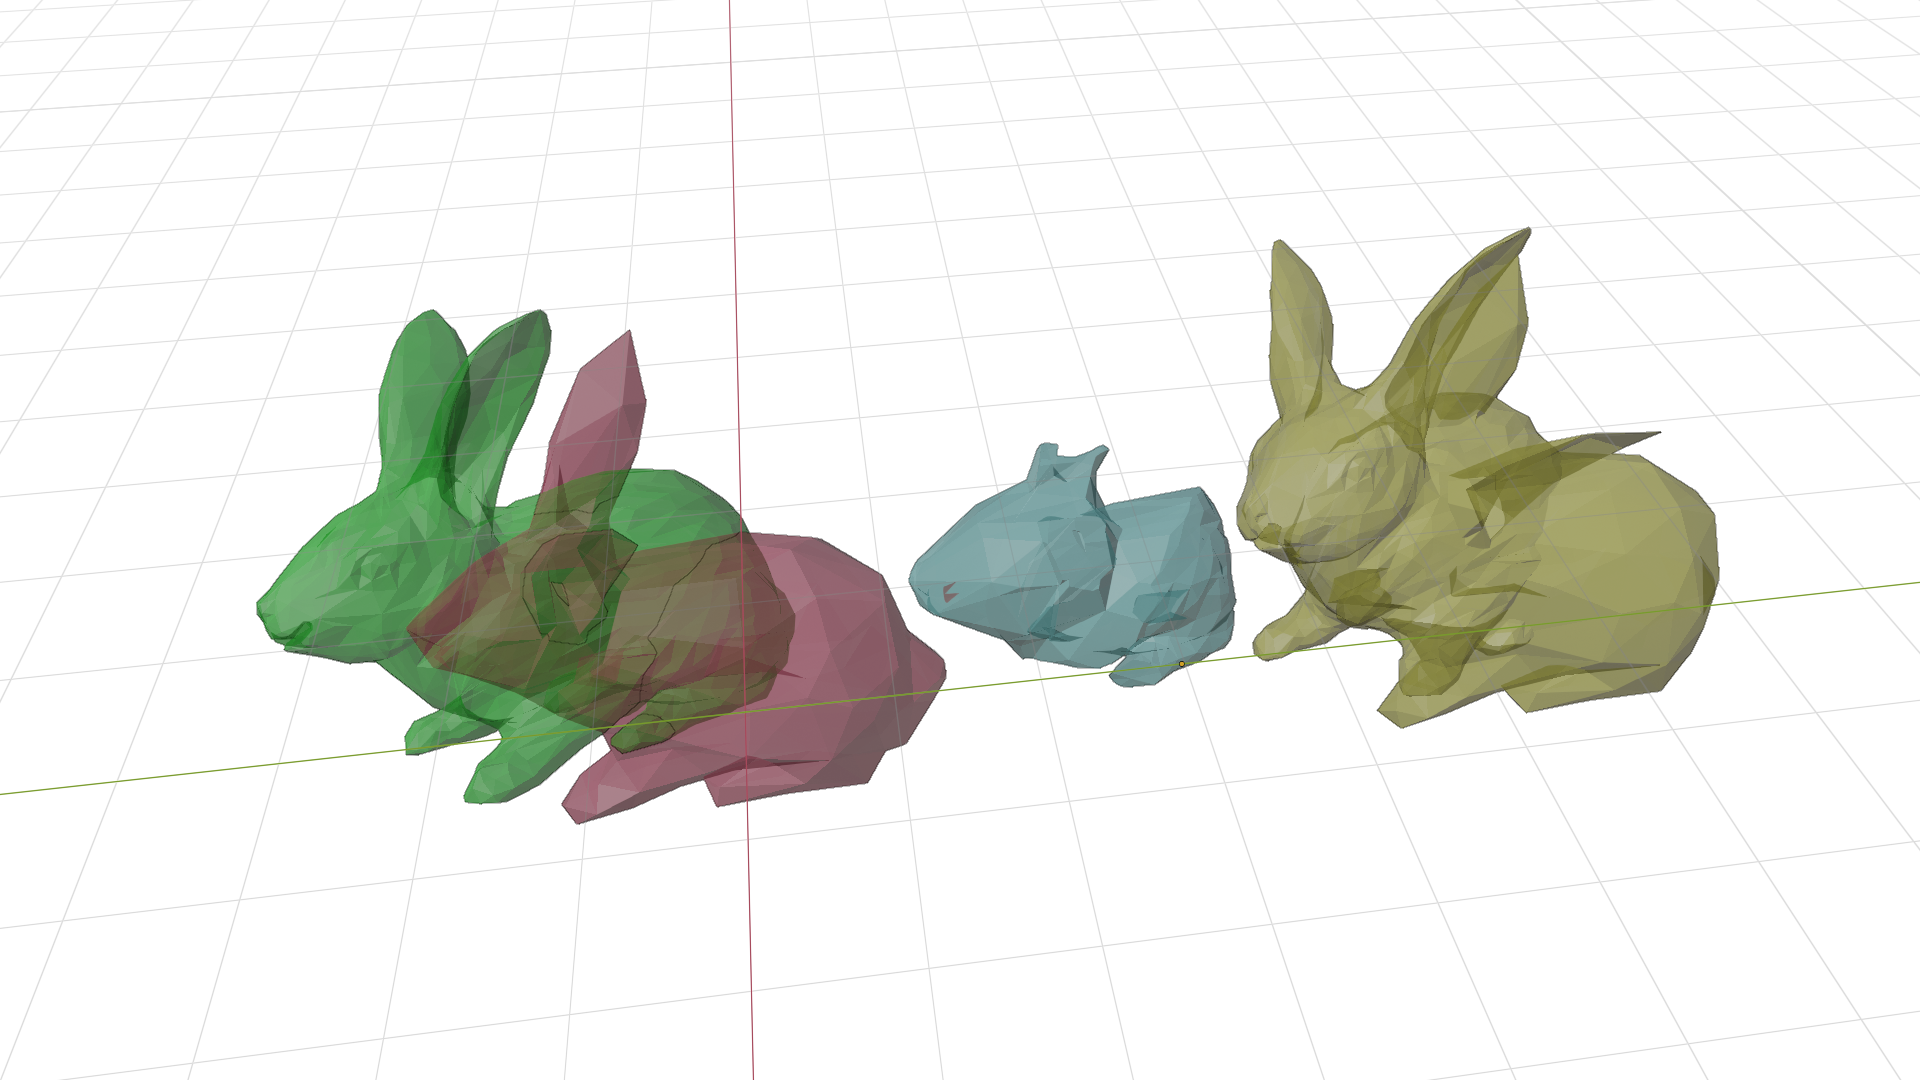
\includegraphics[width = 18cm]{fig/s3s1.png}
\end{figure}

% \subsection{Rabbit and teddy}
\begin{figure}
    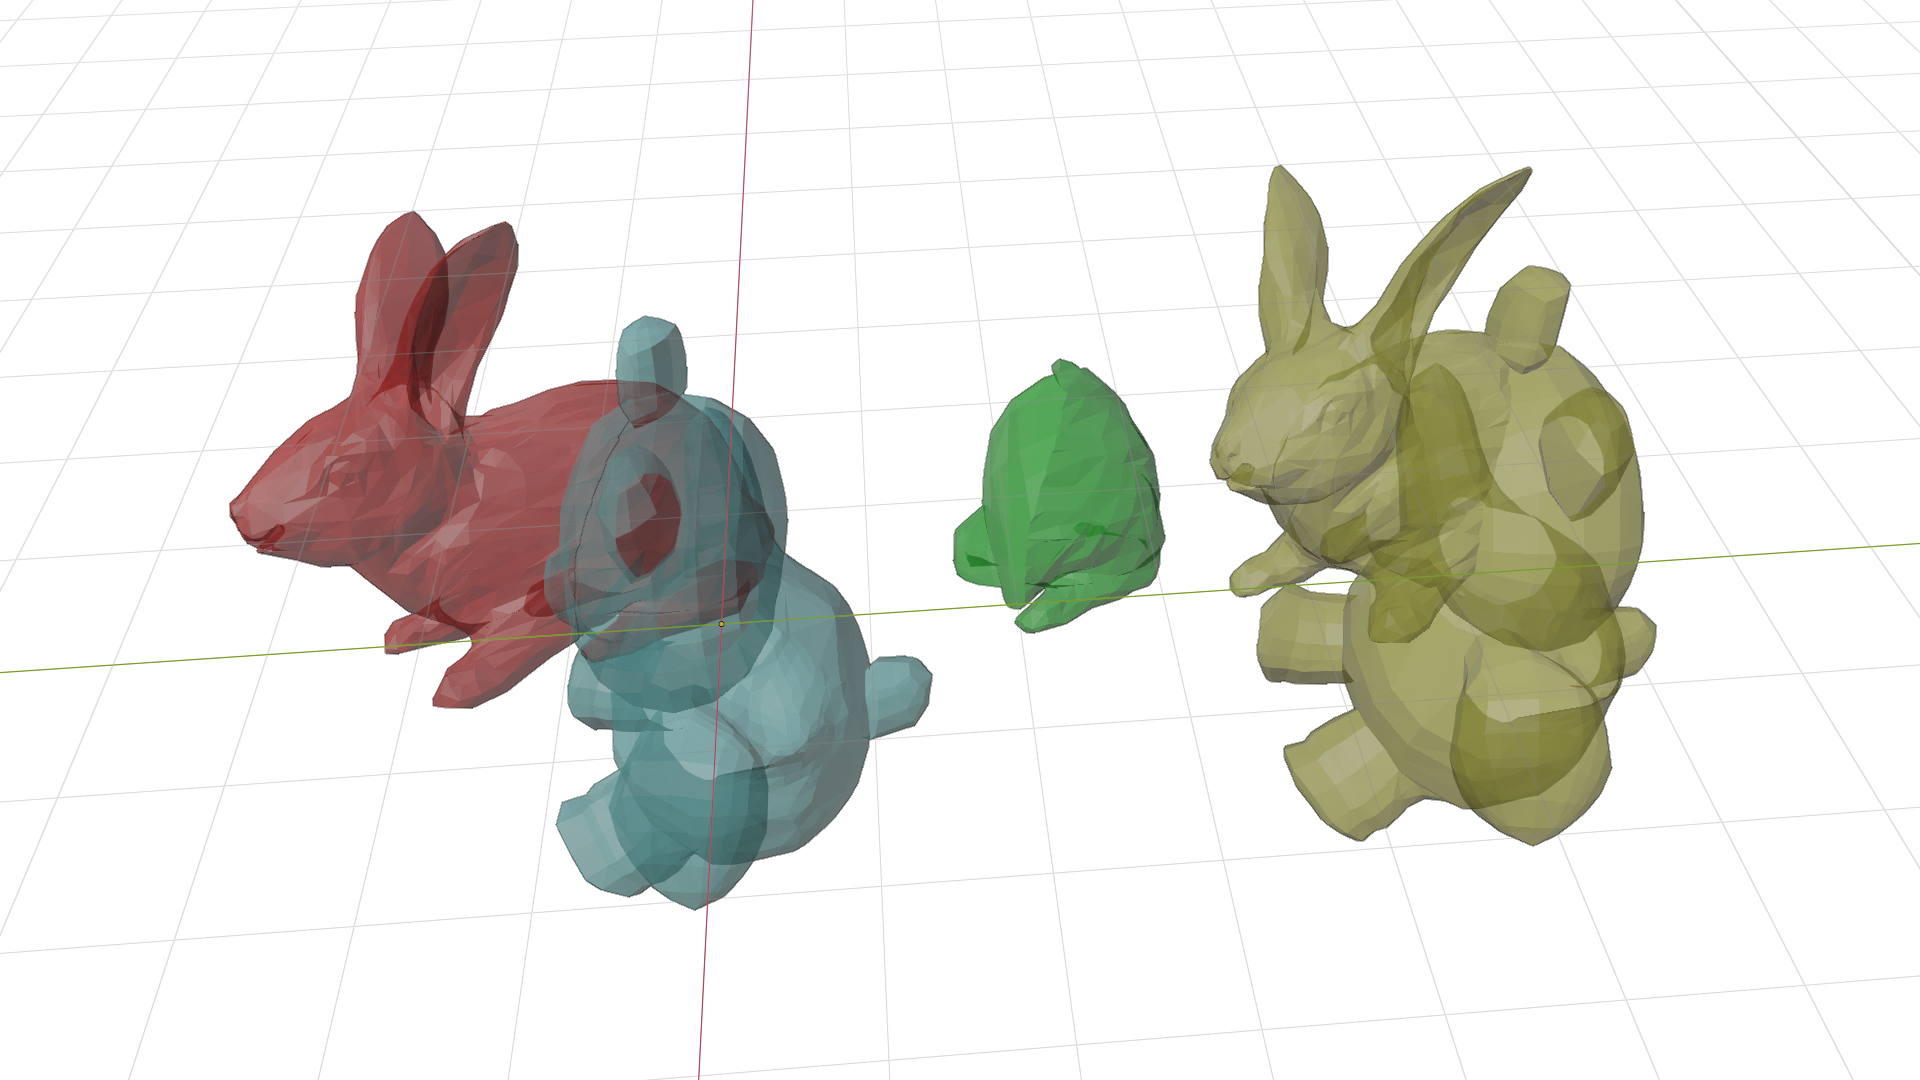
\includegraphics[width = 18cm]{fig/s3s2.png}
\end{figure}

\section{复杂拓扑结构算例}
% \subsection{Torus contain a sphere}
\begin{figure}
    \caption{Bounded green torus meet unbounded blue sphere get right result.}
    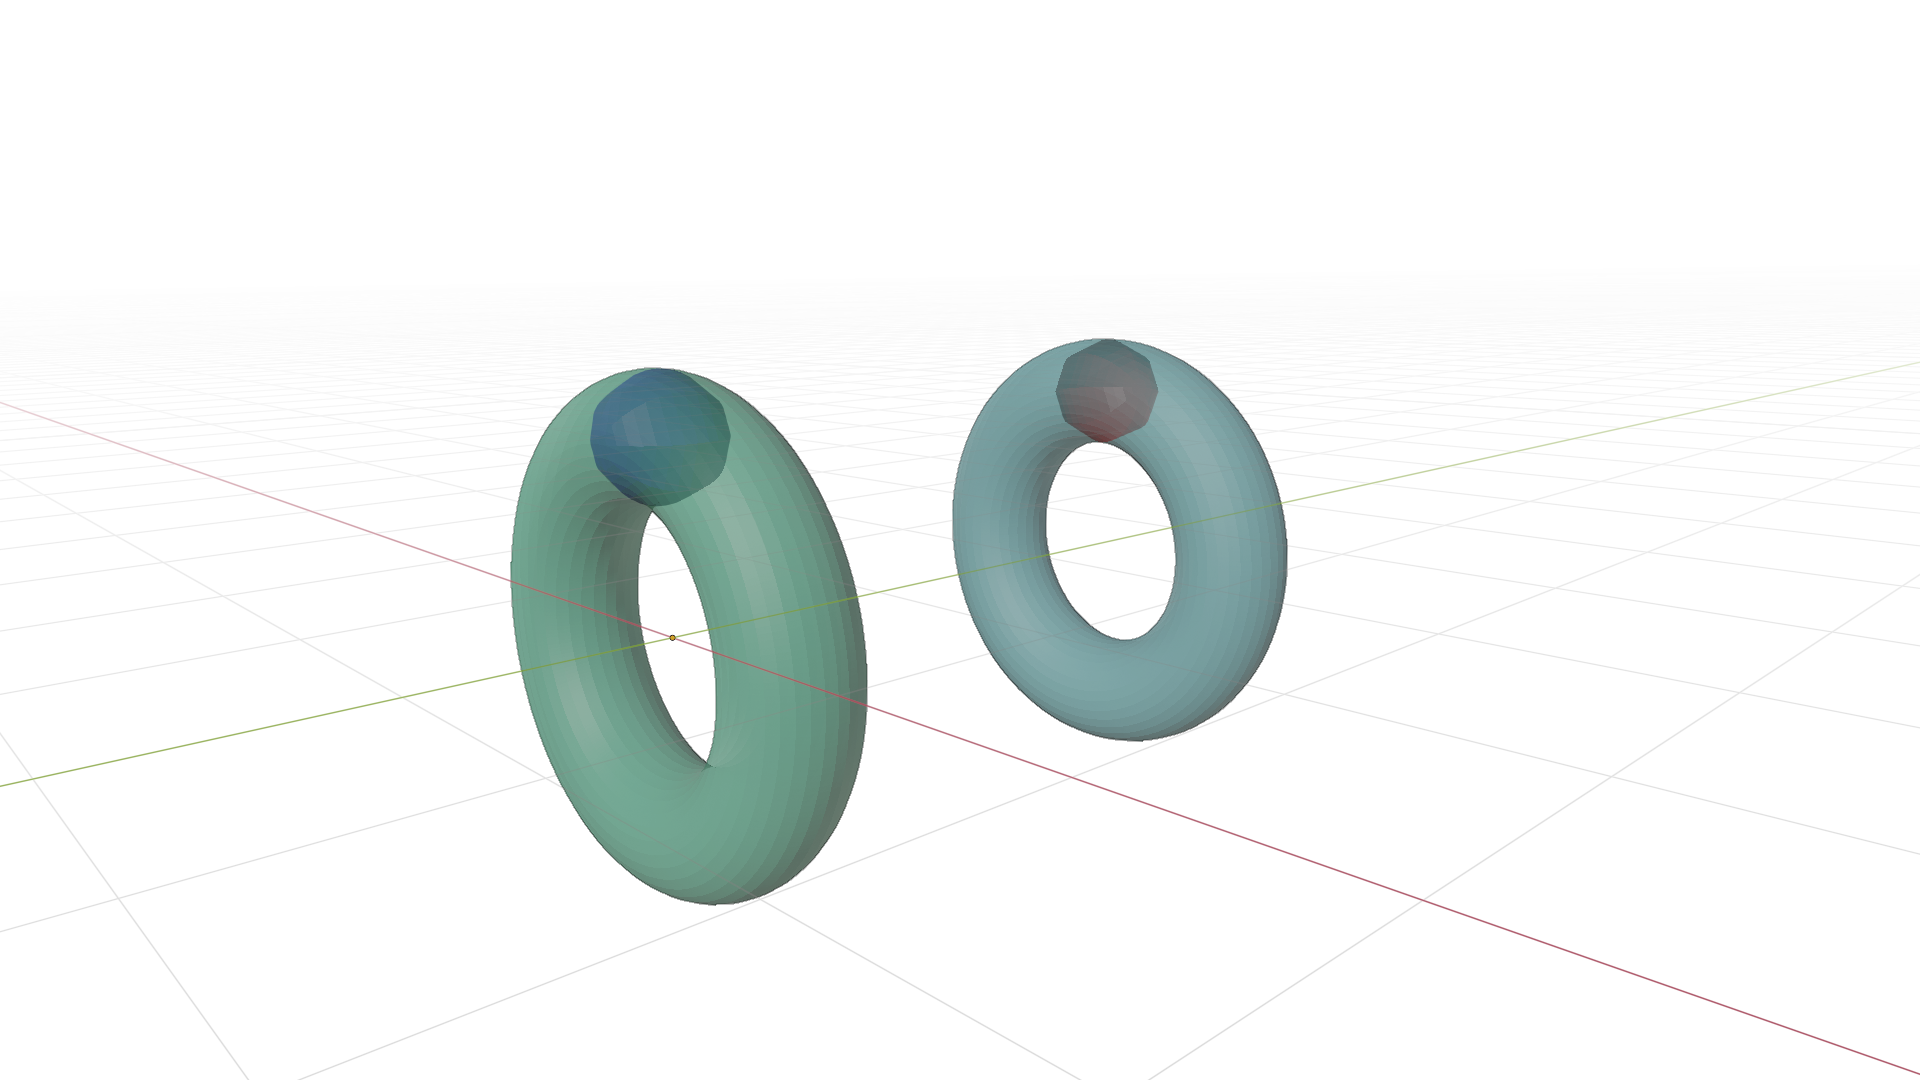
\includegraphics[width = 18cm]{fig/s3s3.png}
\end{figure}

% \subsection{Torus contain two spheres}
\begin{figure}
    \caption{Bounded green torus meet unbounded blue spheres.}
    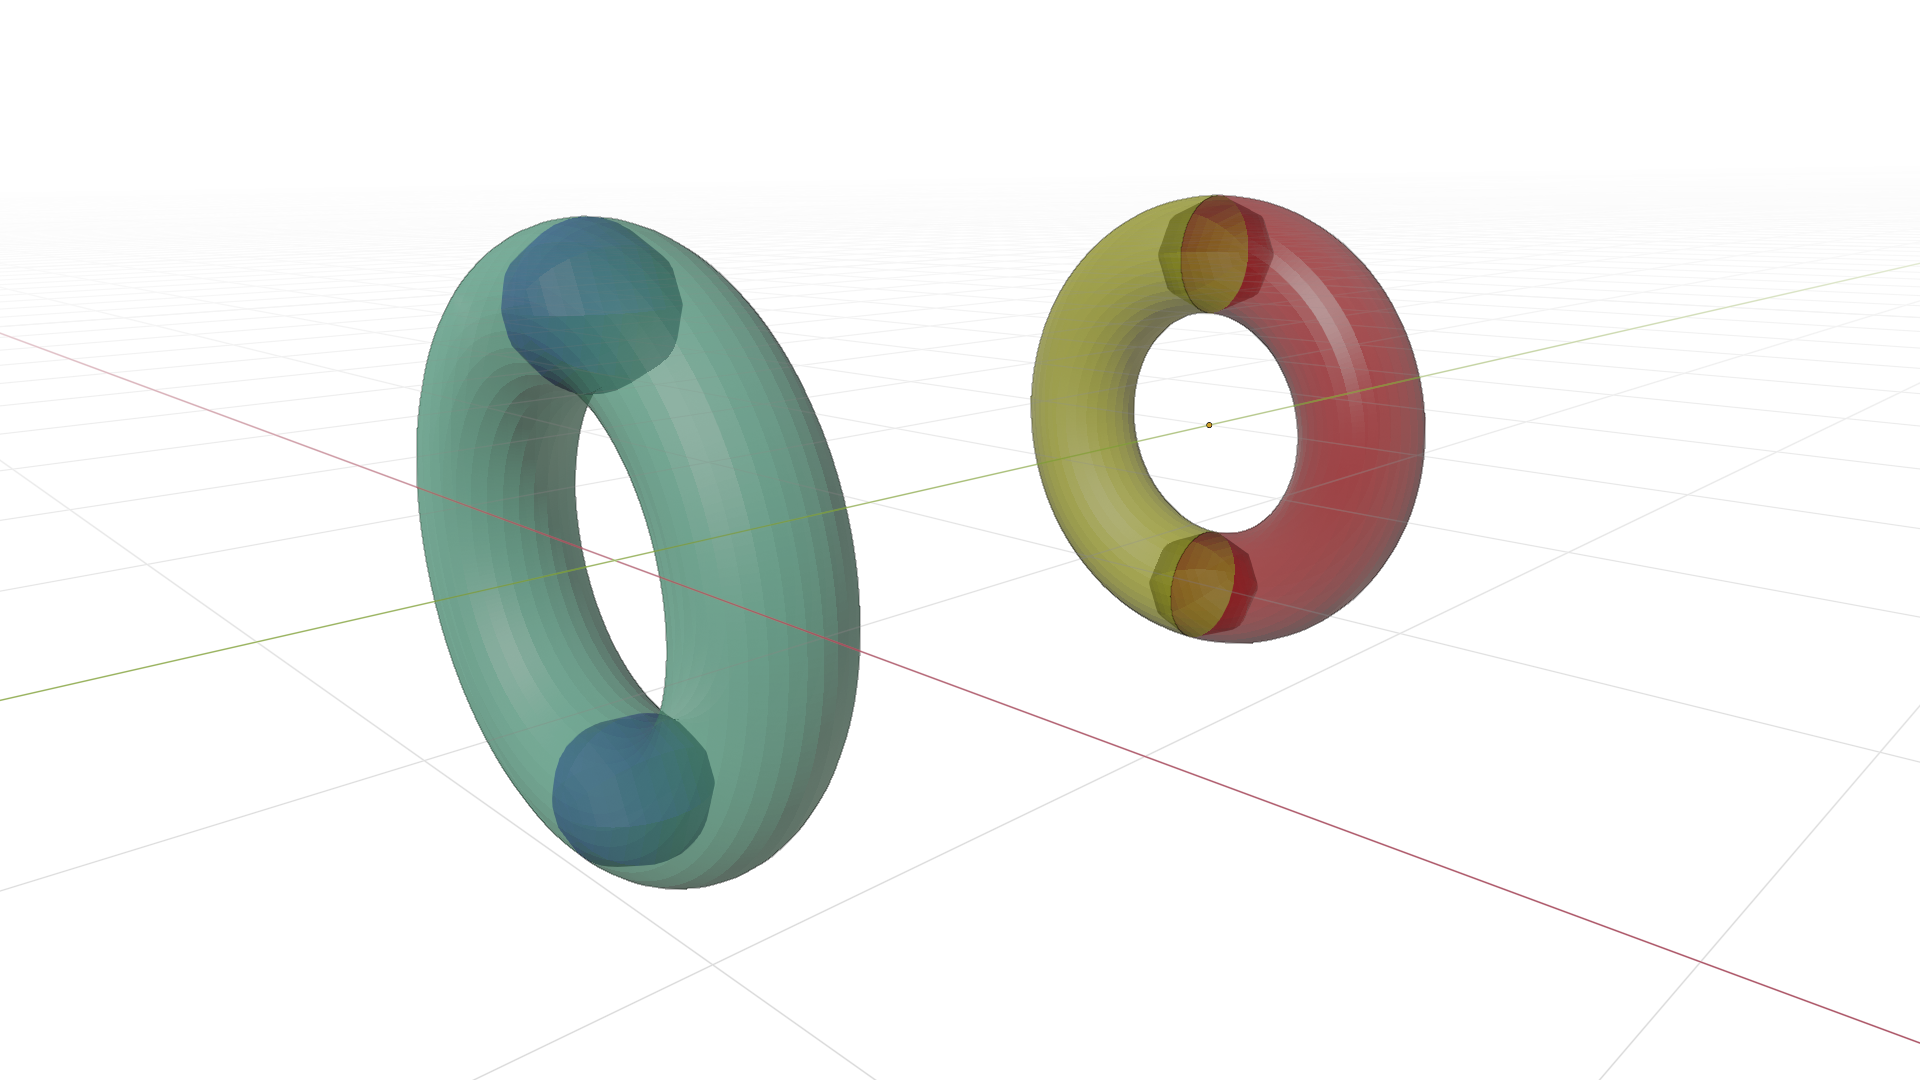
\includegraphics[width = 18cm]{fig/s3s4.png}
\end{figure}

% \subsection{Torus contain sphere connect small torus}
\begin{figure}
    \caption{Bounded cyan torus meet unbounded red sphere connect torus.}
    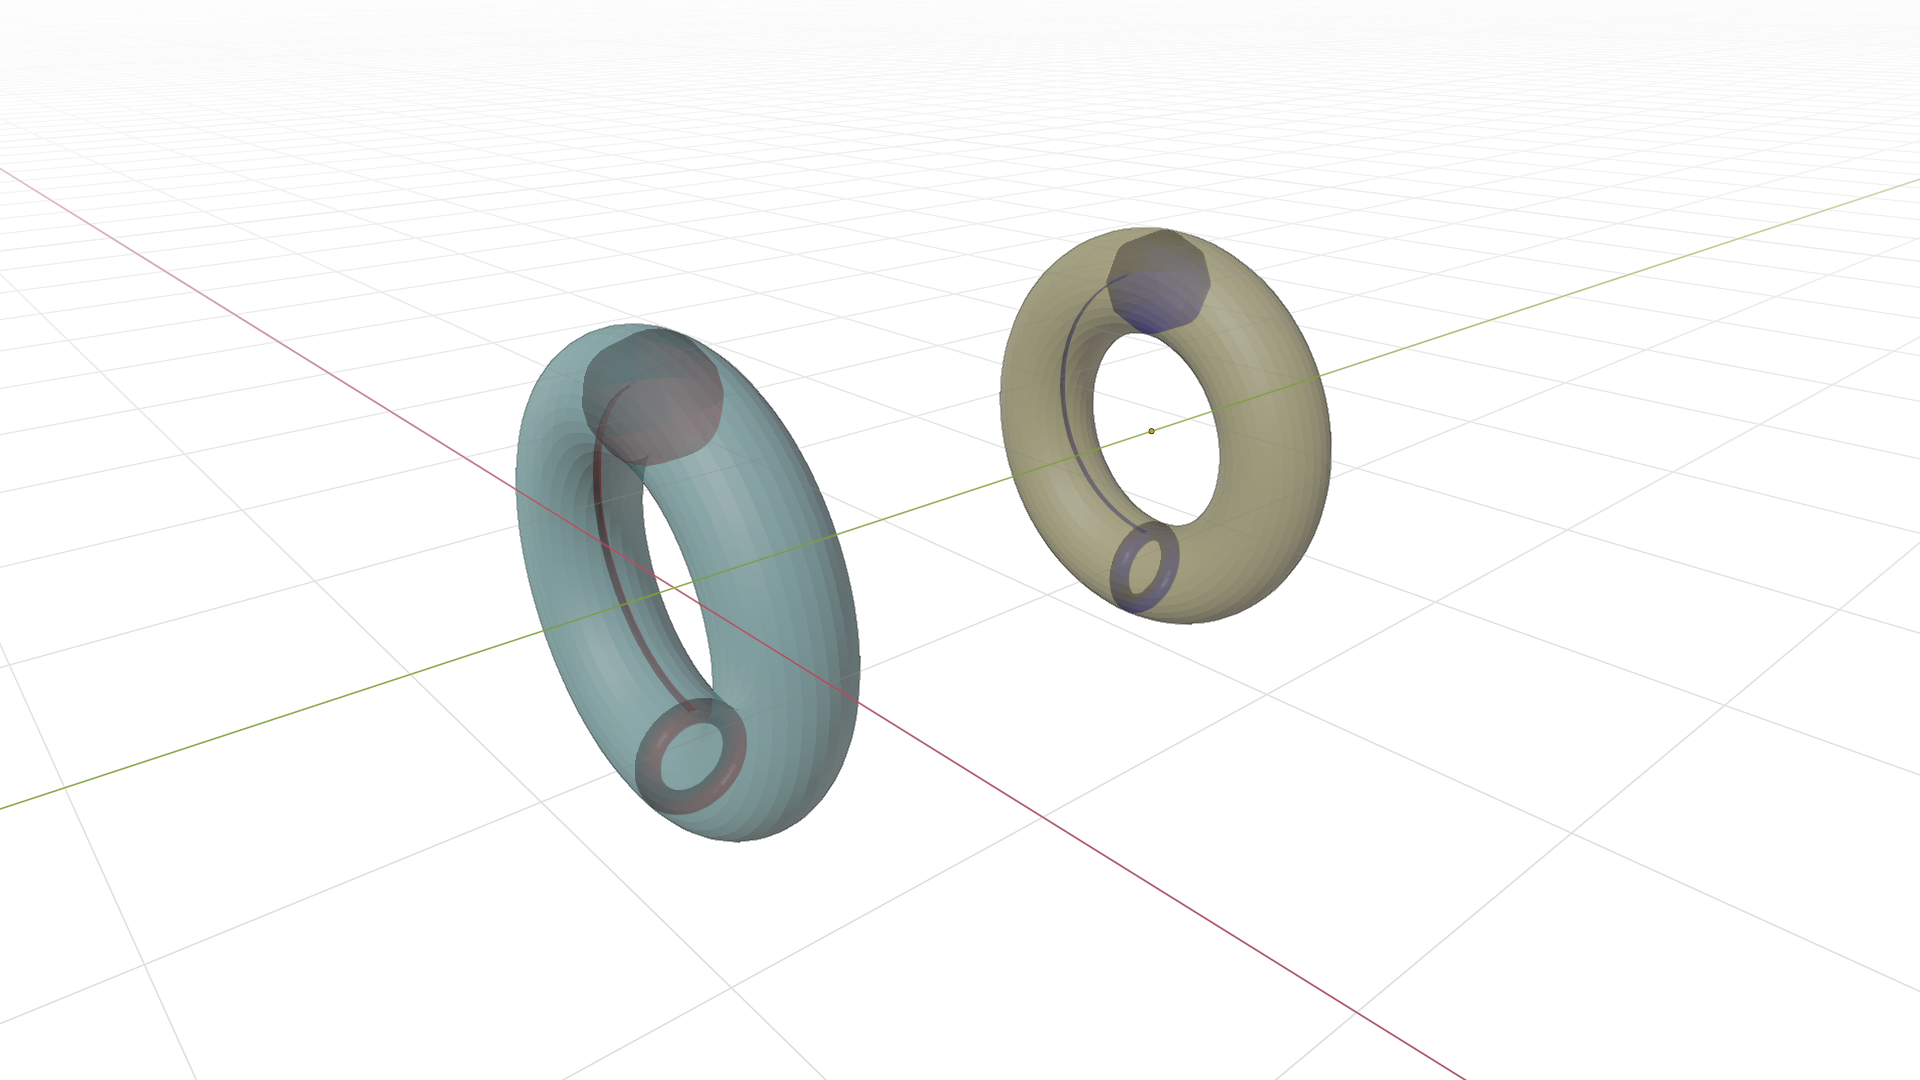
\includegraphics[width = 18cm]{fig/s3s5.png}
\end{figure}

% \subsection{Torus contain a torus }
\begin{figure}
    \caption{Bounded cyan torus meet unbounded red torus.}
    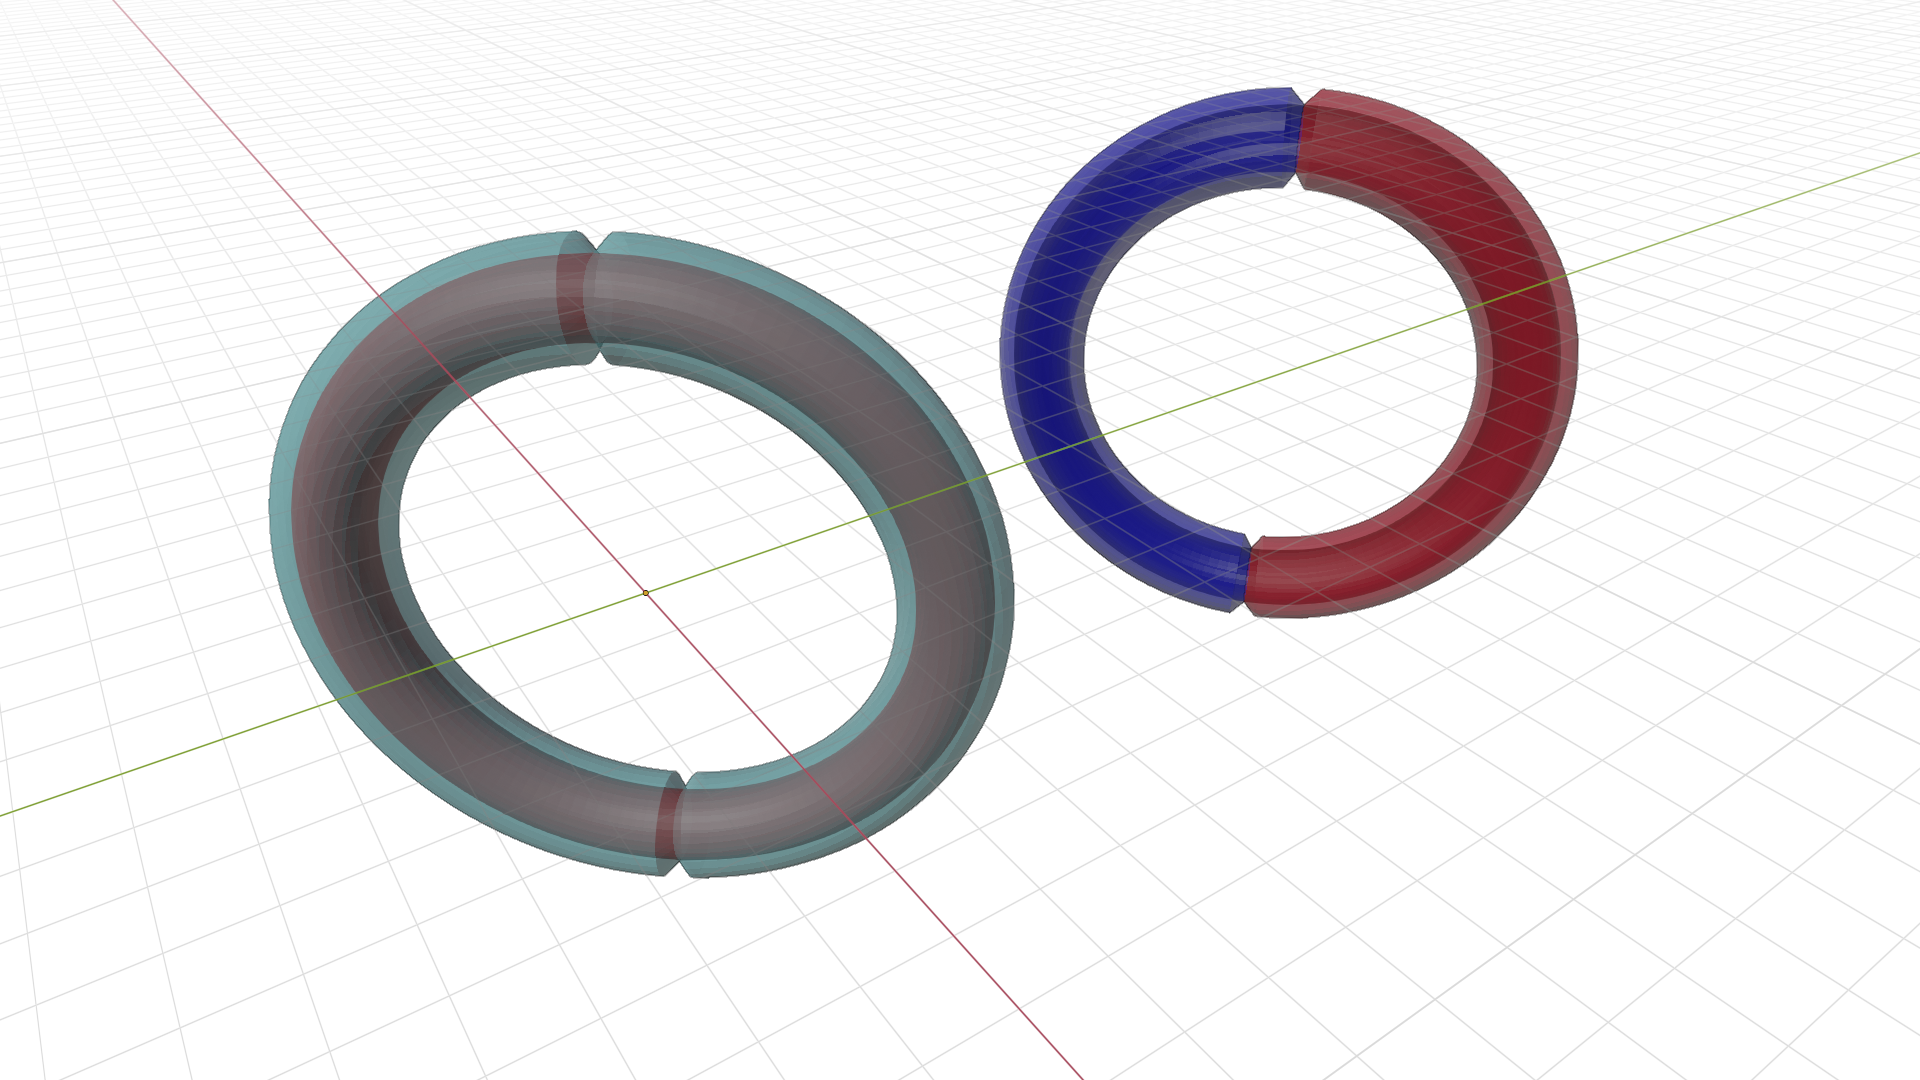
\includegraphics[width = 18cm]{fig/s3s6.png}
\end{figure}


% \section{几个定义}
% GluingCloseSurface,SurfacePatch,需要保留的交线和不需要保留的交线如下图所示.

% \begin{figure}
%     \caption{GluingCompactSurface}
%     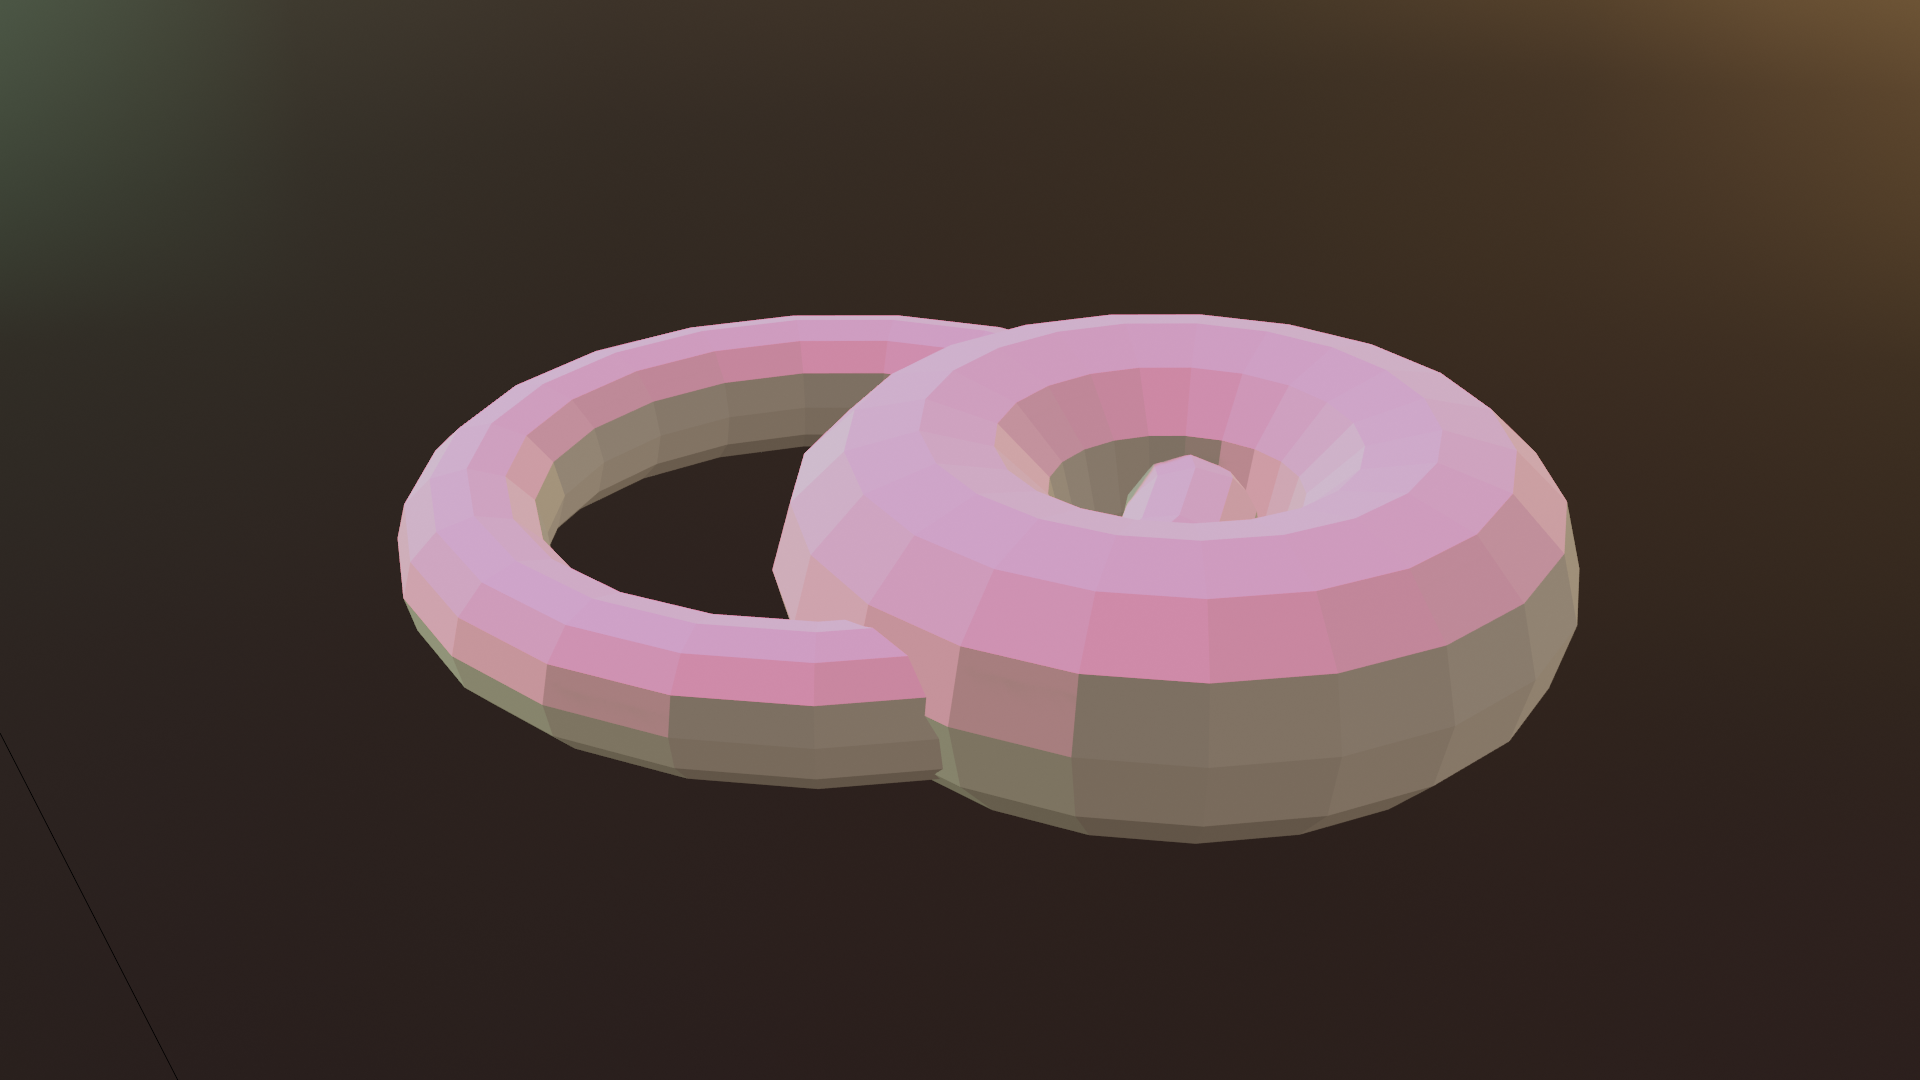
\includegraphics[width = 18cm]{fig/GluingCompactSurface1.png}
%     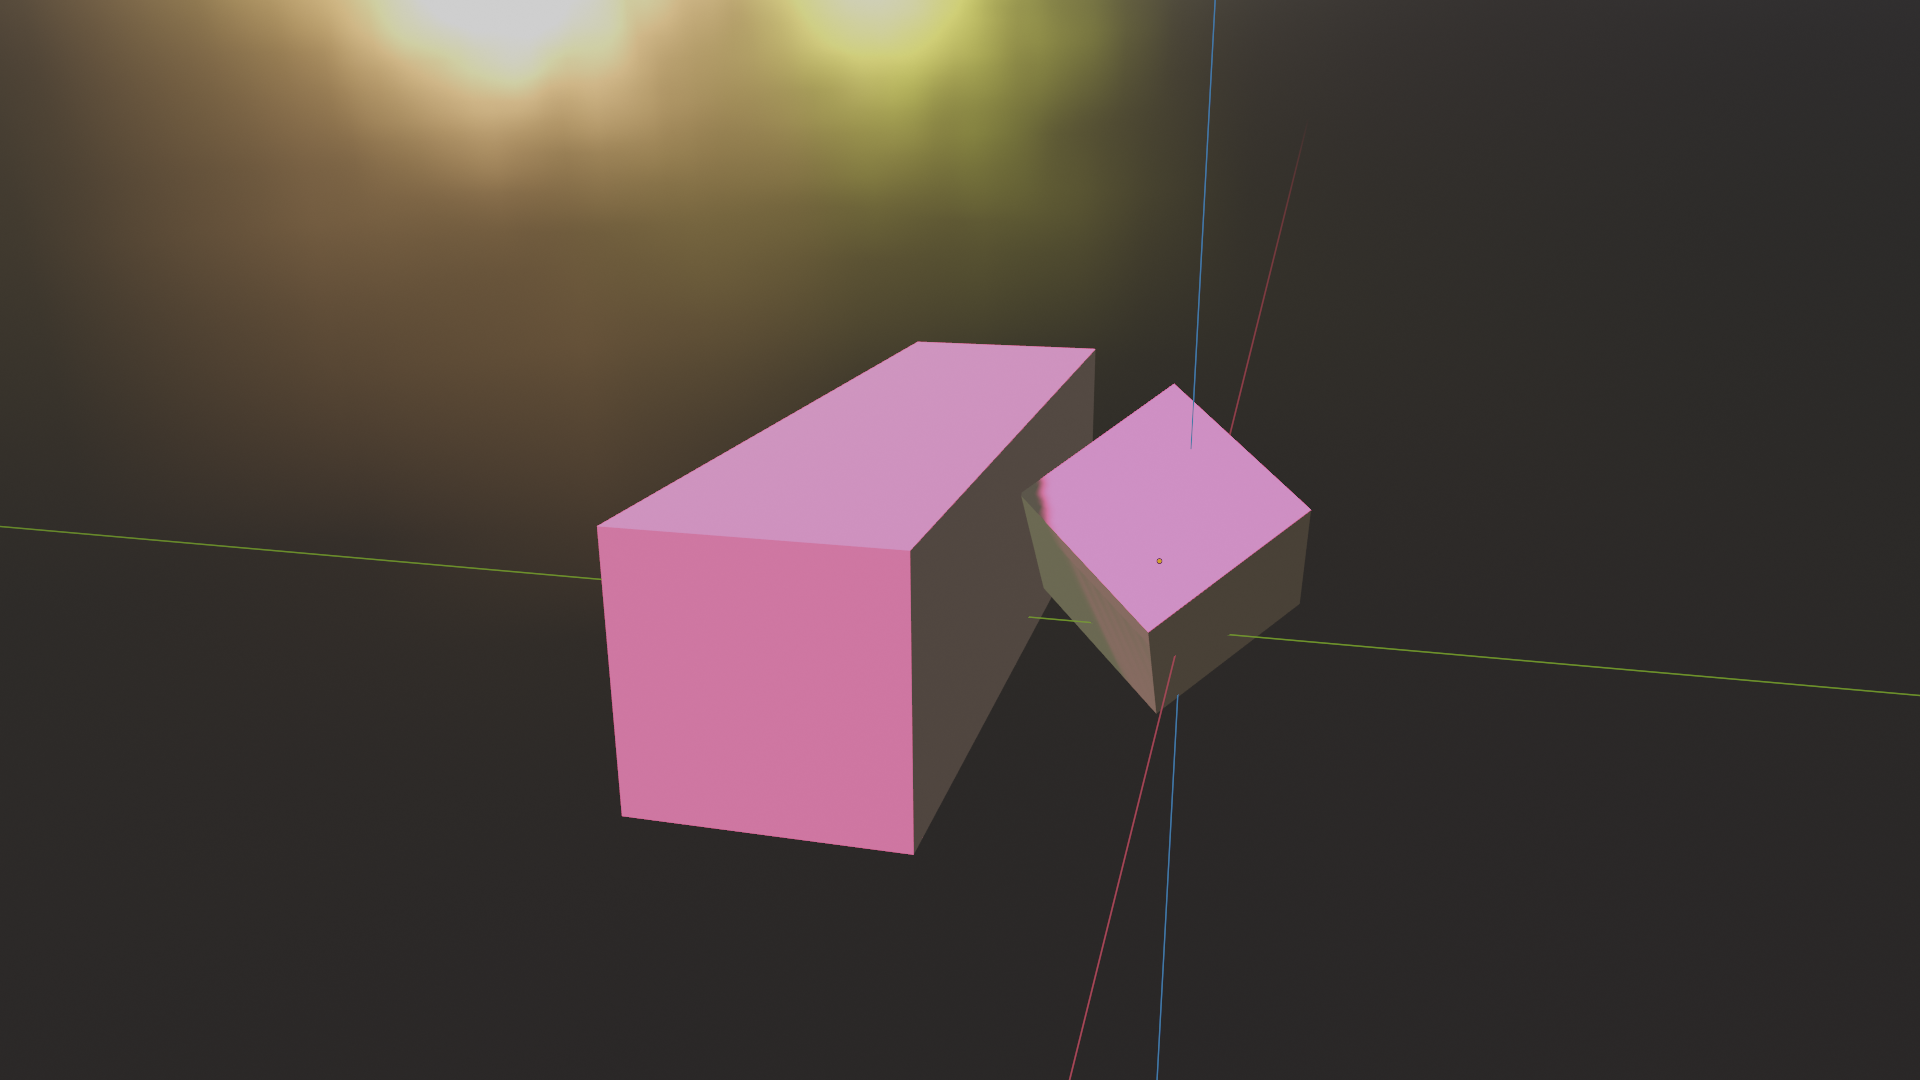
\includegraphics[width = 18cm]{fig/GluingCompactSurface2.png}
% \end{figure}

% \begin{figure}
%     \caption{SurfacePatch}
%     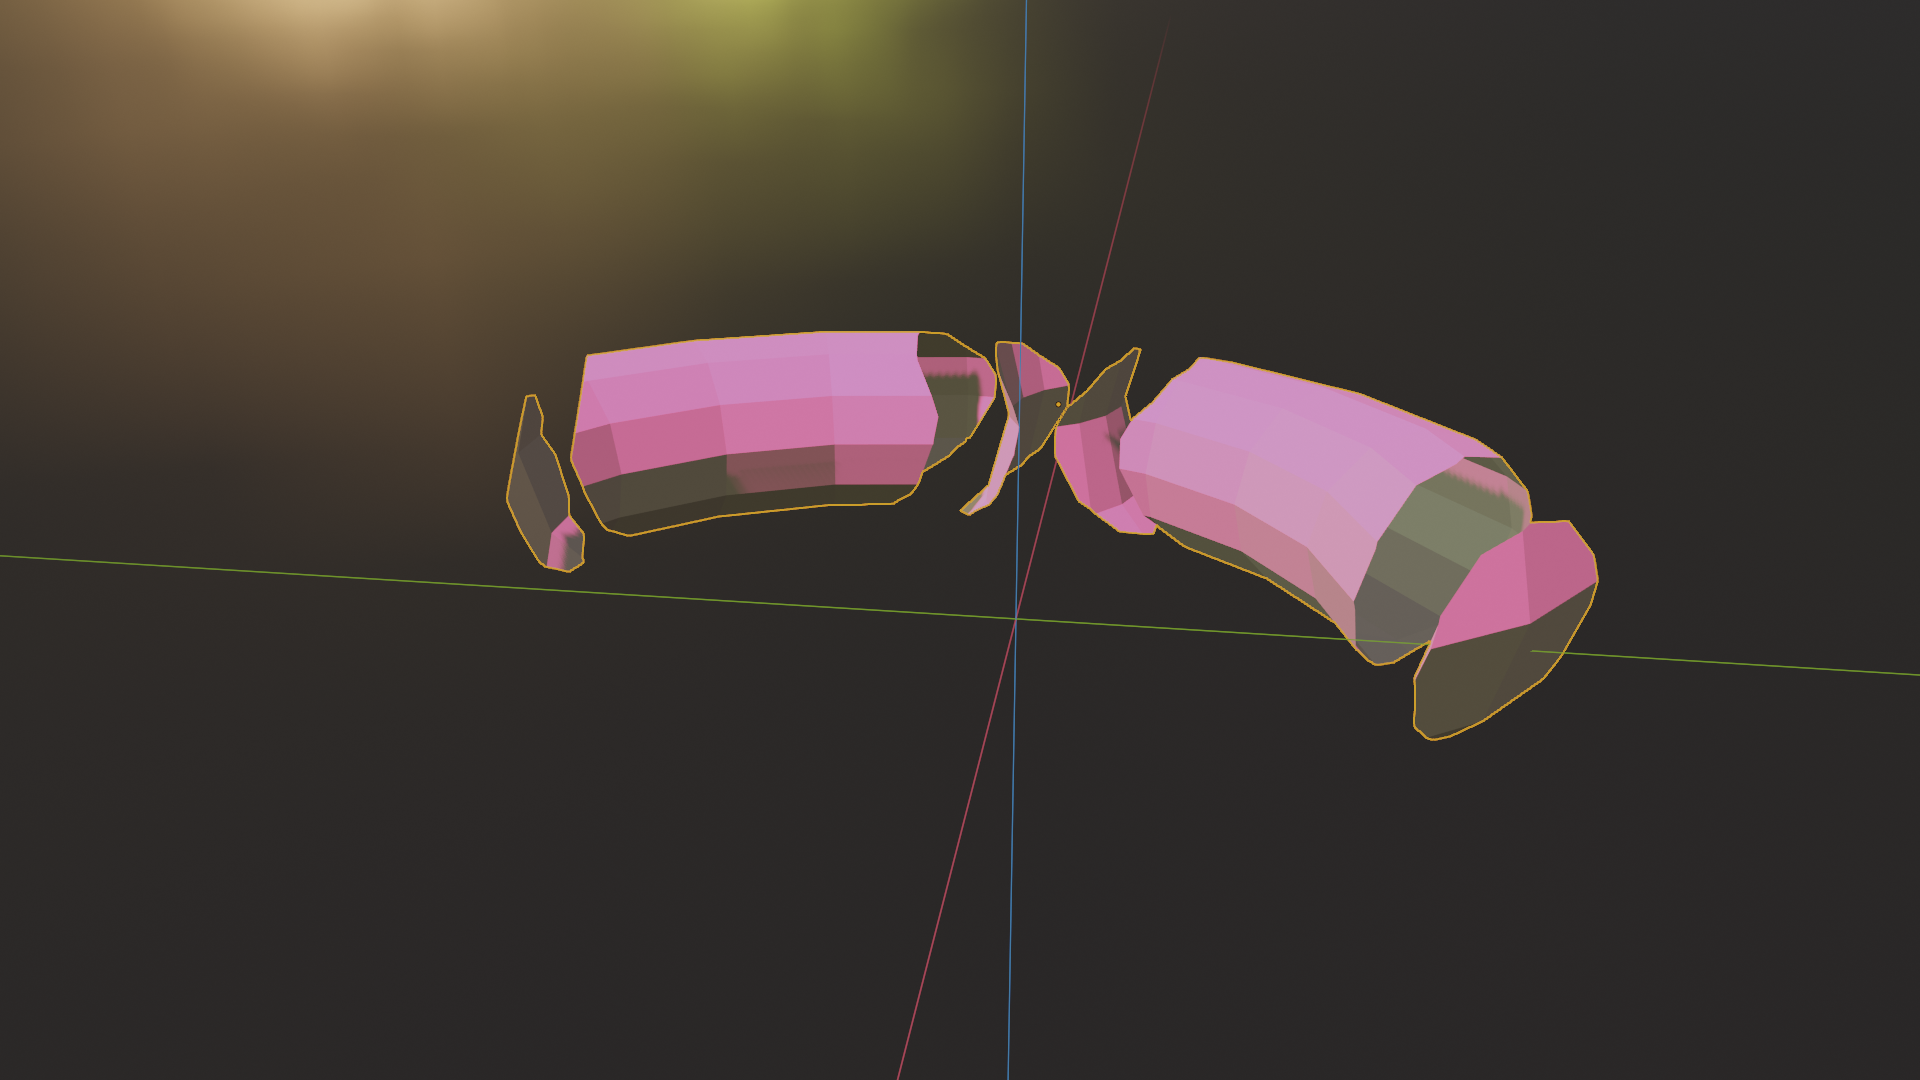
\includegraphics[width = 18cm]{fig/SurfacePatch1.png}
%     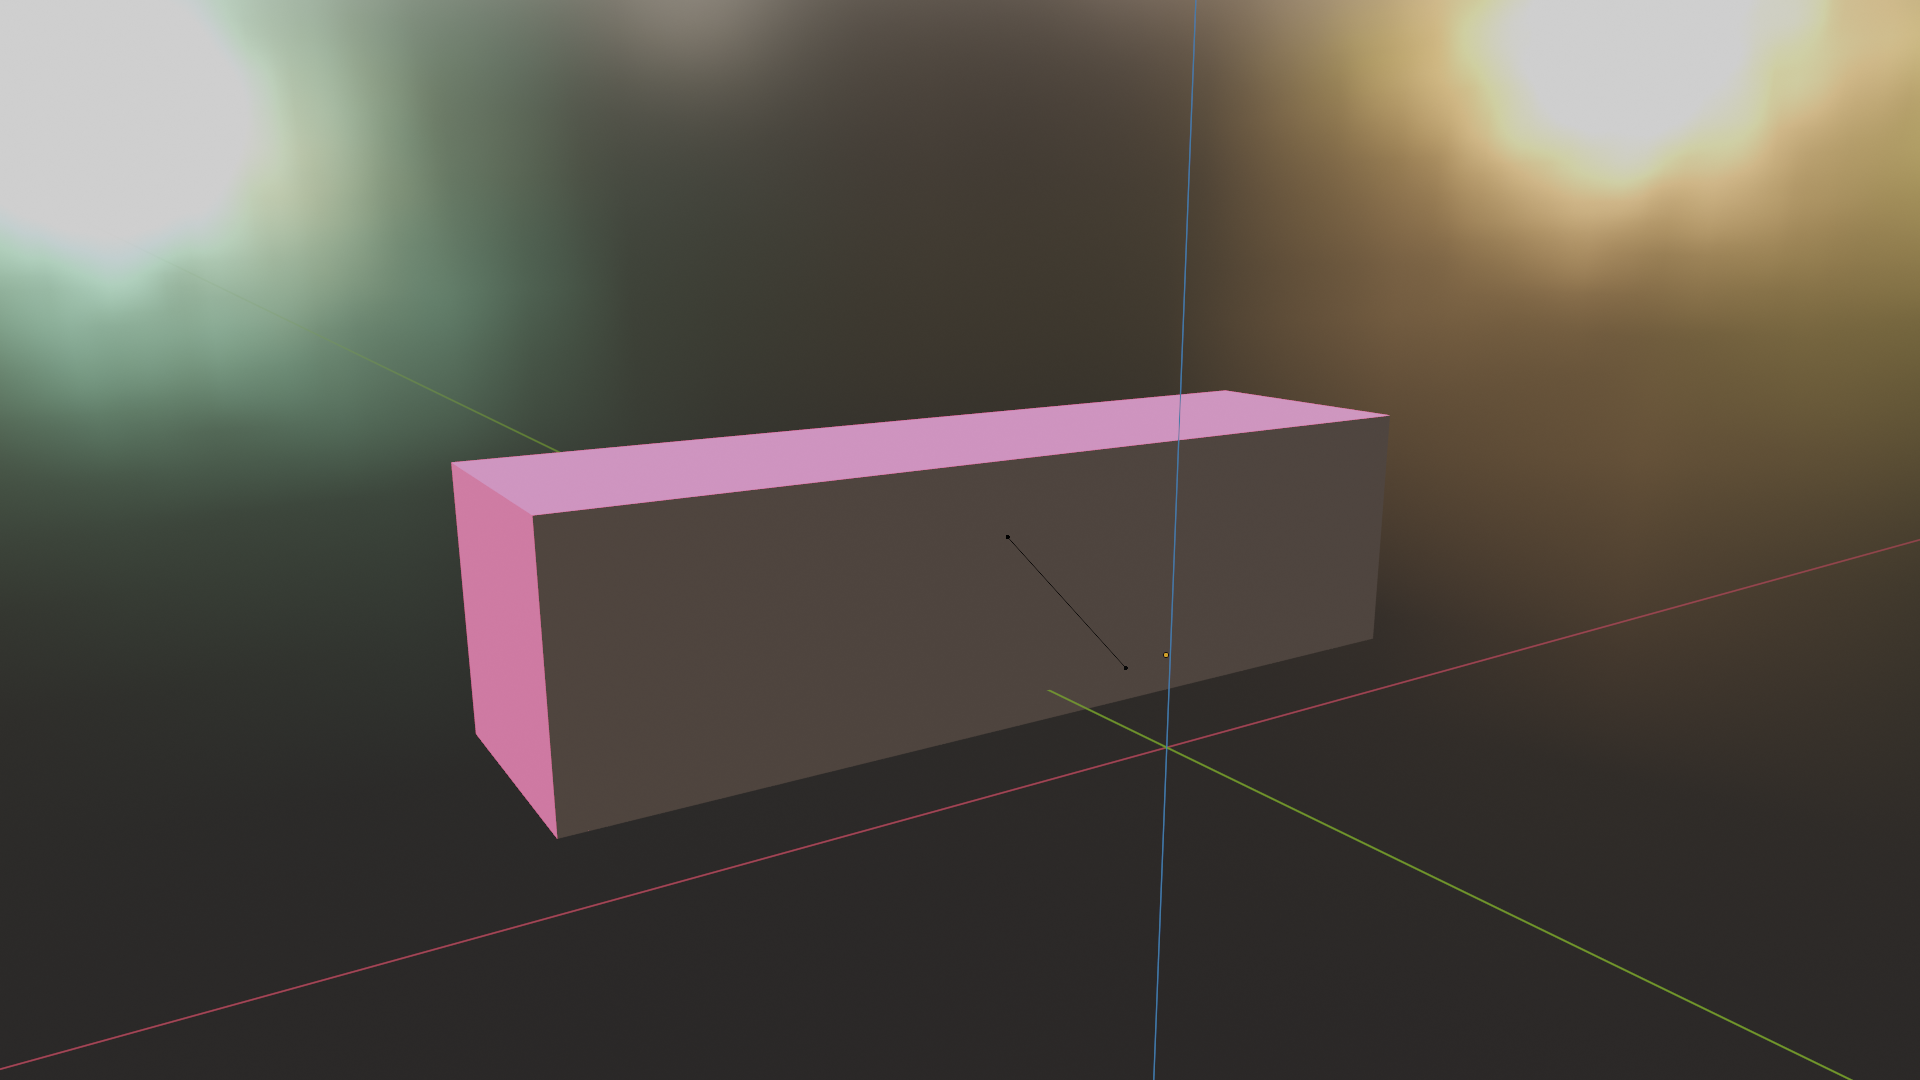
\includegraphics[width = 18cm]{fig/SurfacePatch2.png}
% \end{figure}
% 交线即为每个曲面片的边界线,在torus示例中有6张曲面片,4条交线.长方体示例中只有一张曲面片,
% 一条交线.且torus示例中的交线都同时是两张切割的曲面片的边界,因此都需要保留.在长方体示例
% 中交线只是一个曲面片的边界,所以需要移除.

% \section{其它几个手画处理过程}
% 因为GluingCompactSurface的内部有交时交出的交线必将GluingCompactSurface划分为两个连通分量.
% 所以在这里只考虑里两个连通分量相切时的处理过程.

% \begin{figure}
%     \caption{简单的示范:torus内切一个球}
%     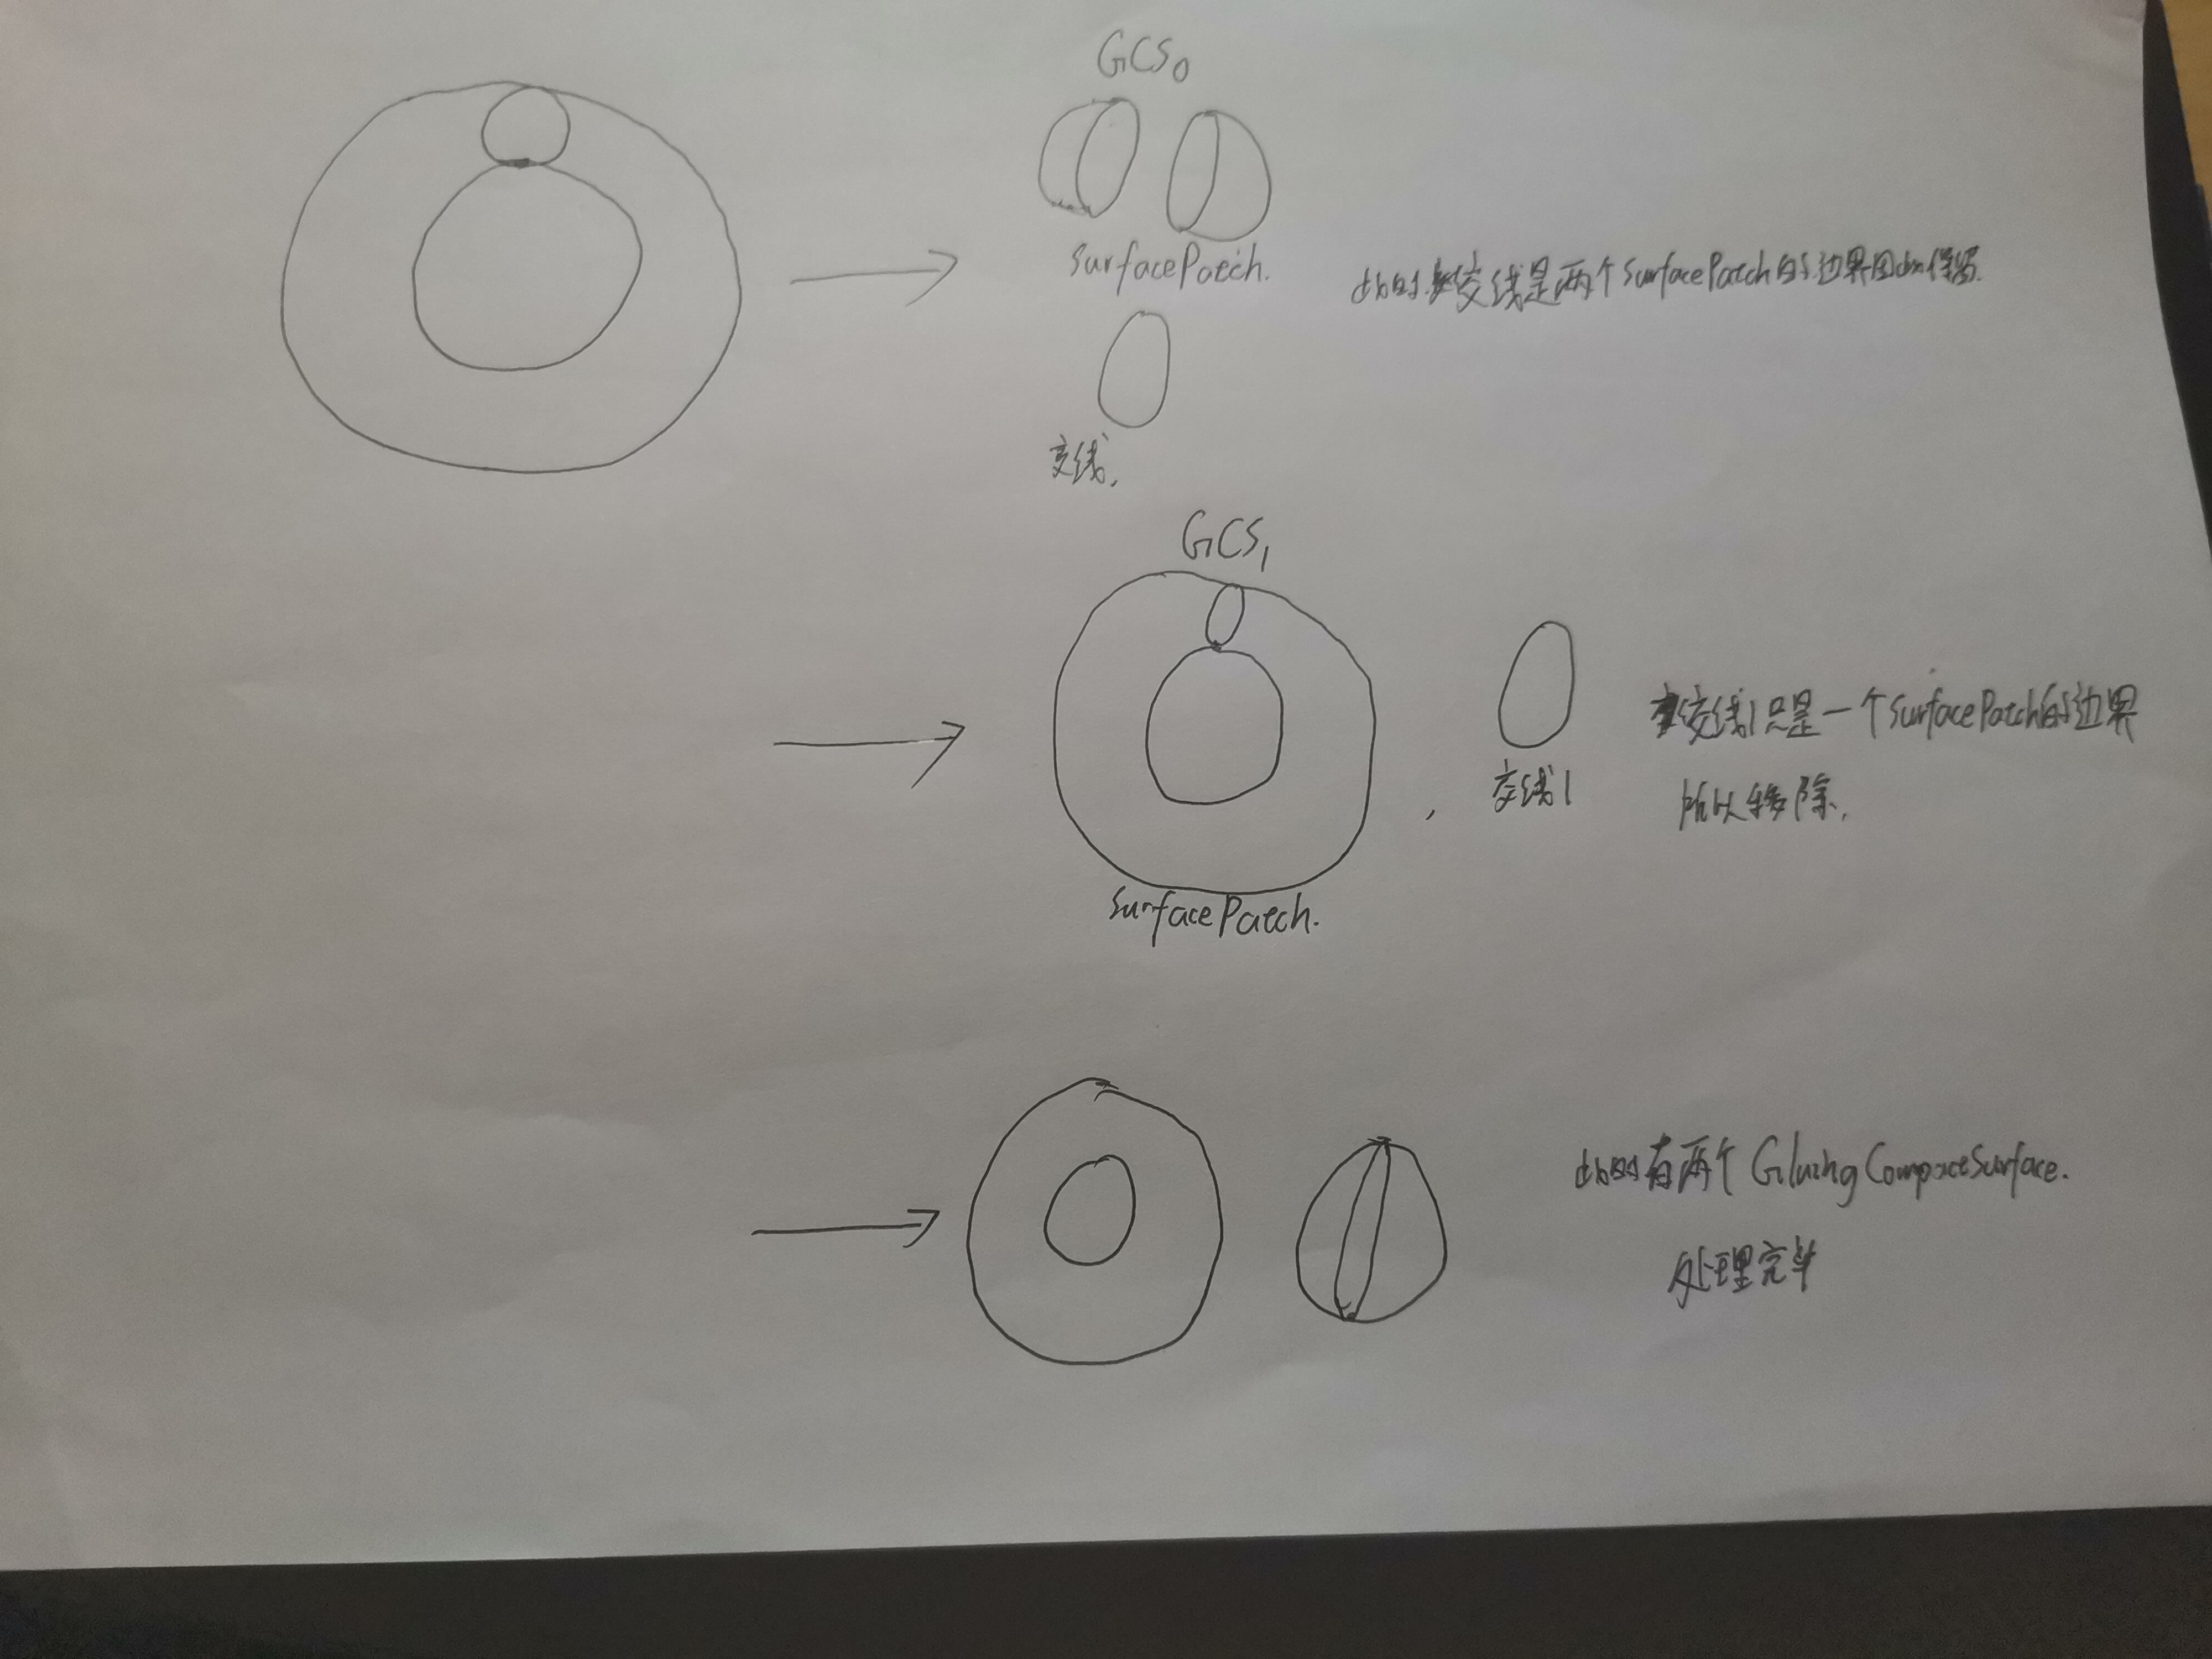
\includegraphics[width = 18cm]{fig/writing0.jpg}
% \end{figure}

% \begin{figure}
%     \caption{交线不为闭合曲线时}
%     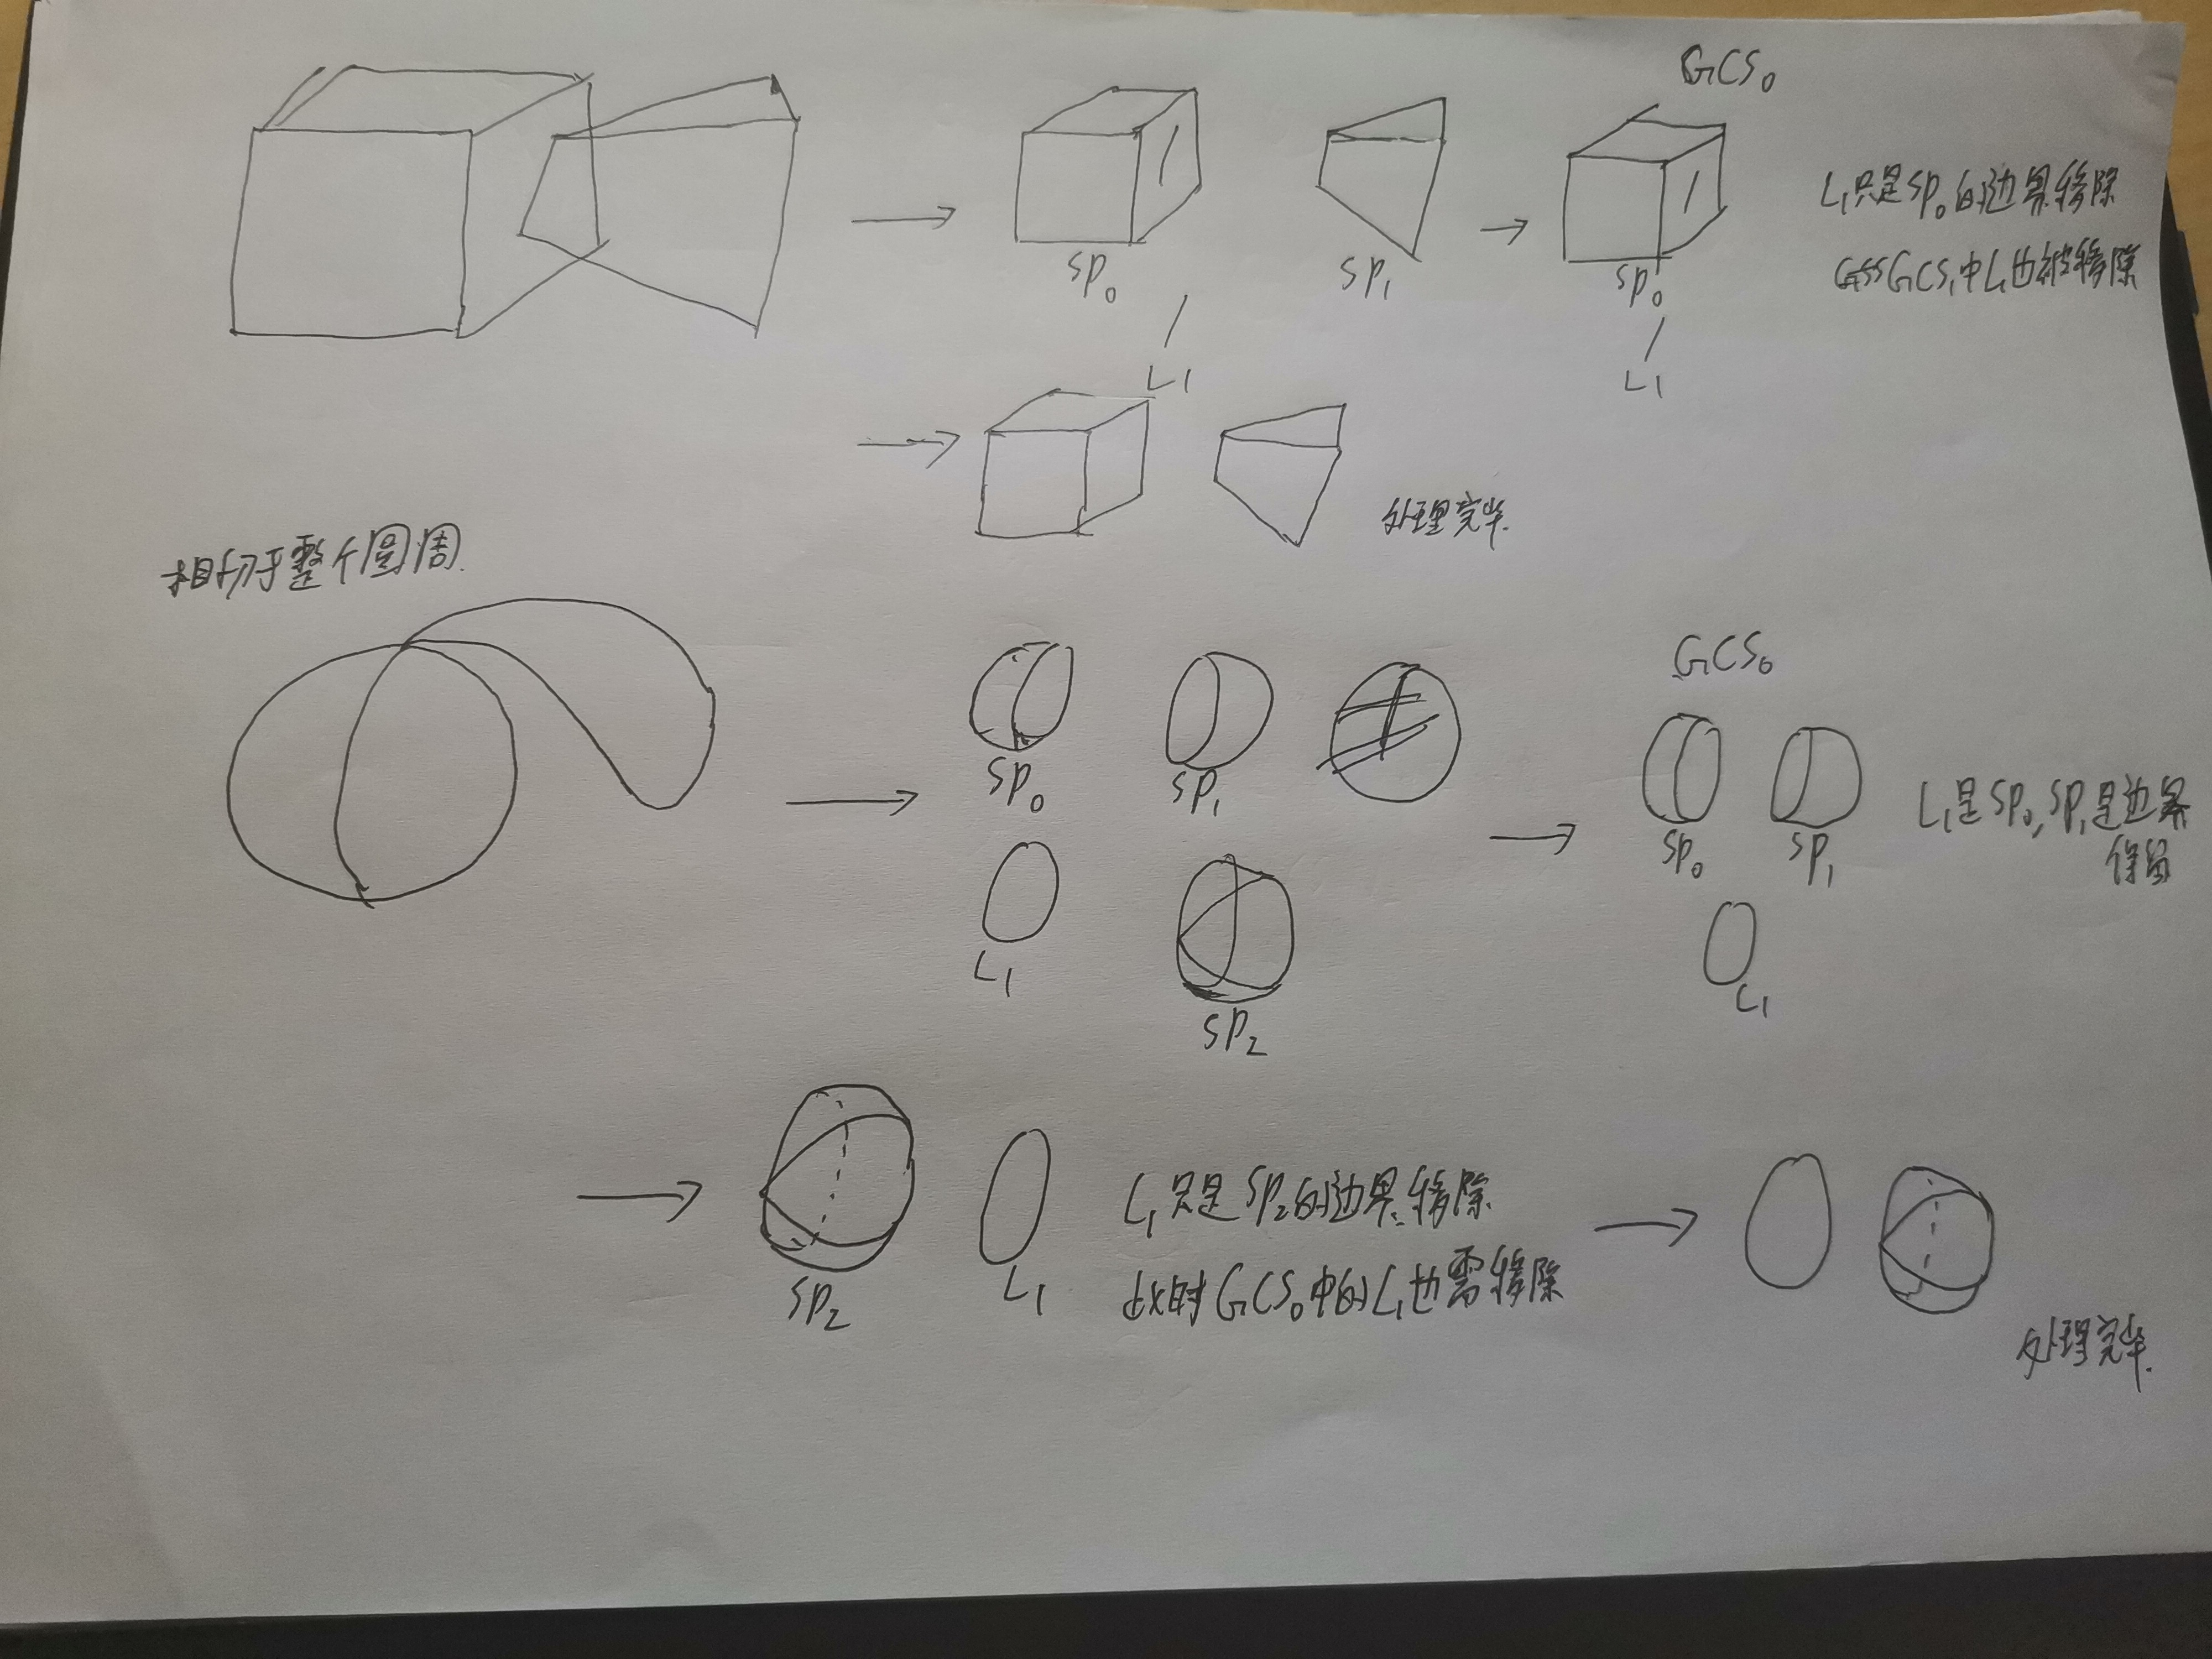
\includegraphics[width = 18cm]{fig/writing1.jpg}
% \end{figure}

% \begin{figure}
%     \caption{torus内切两个球}
%     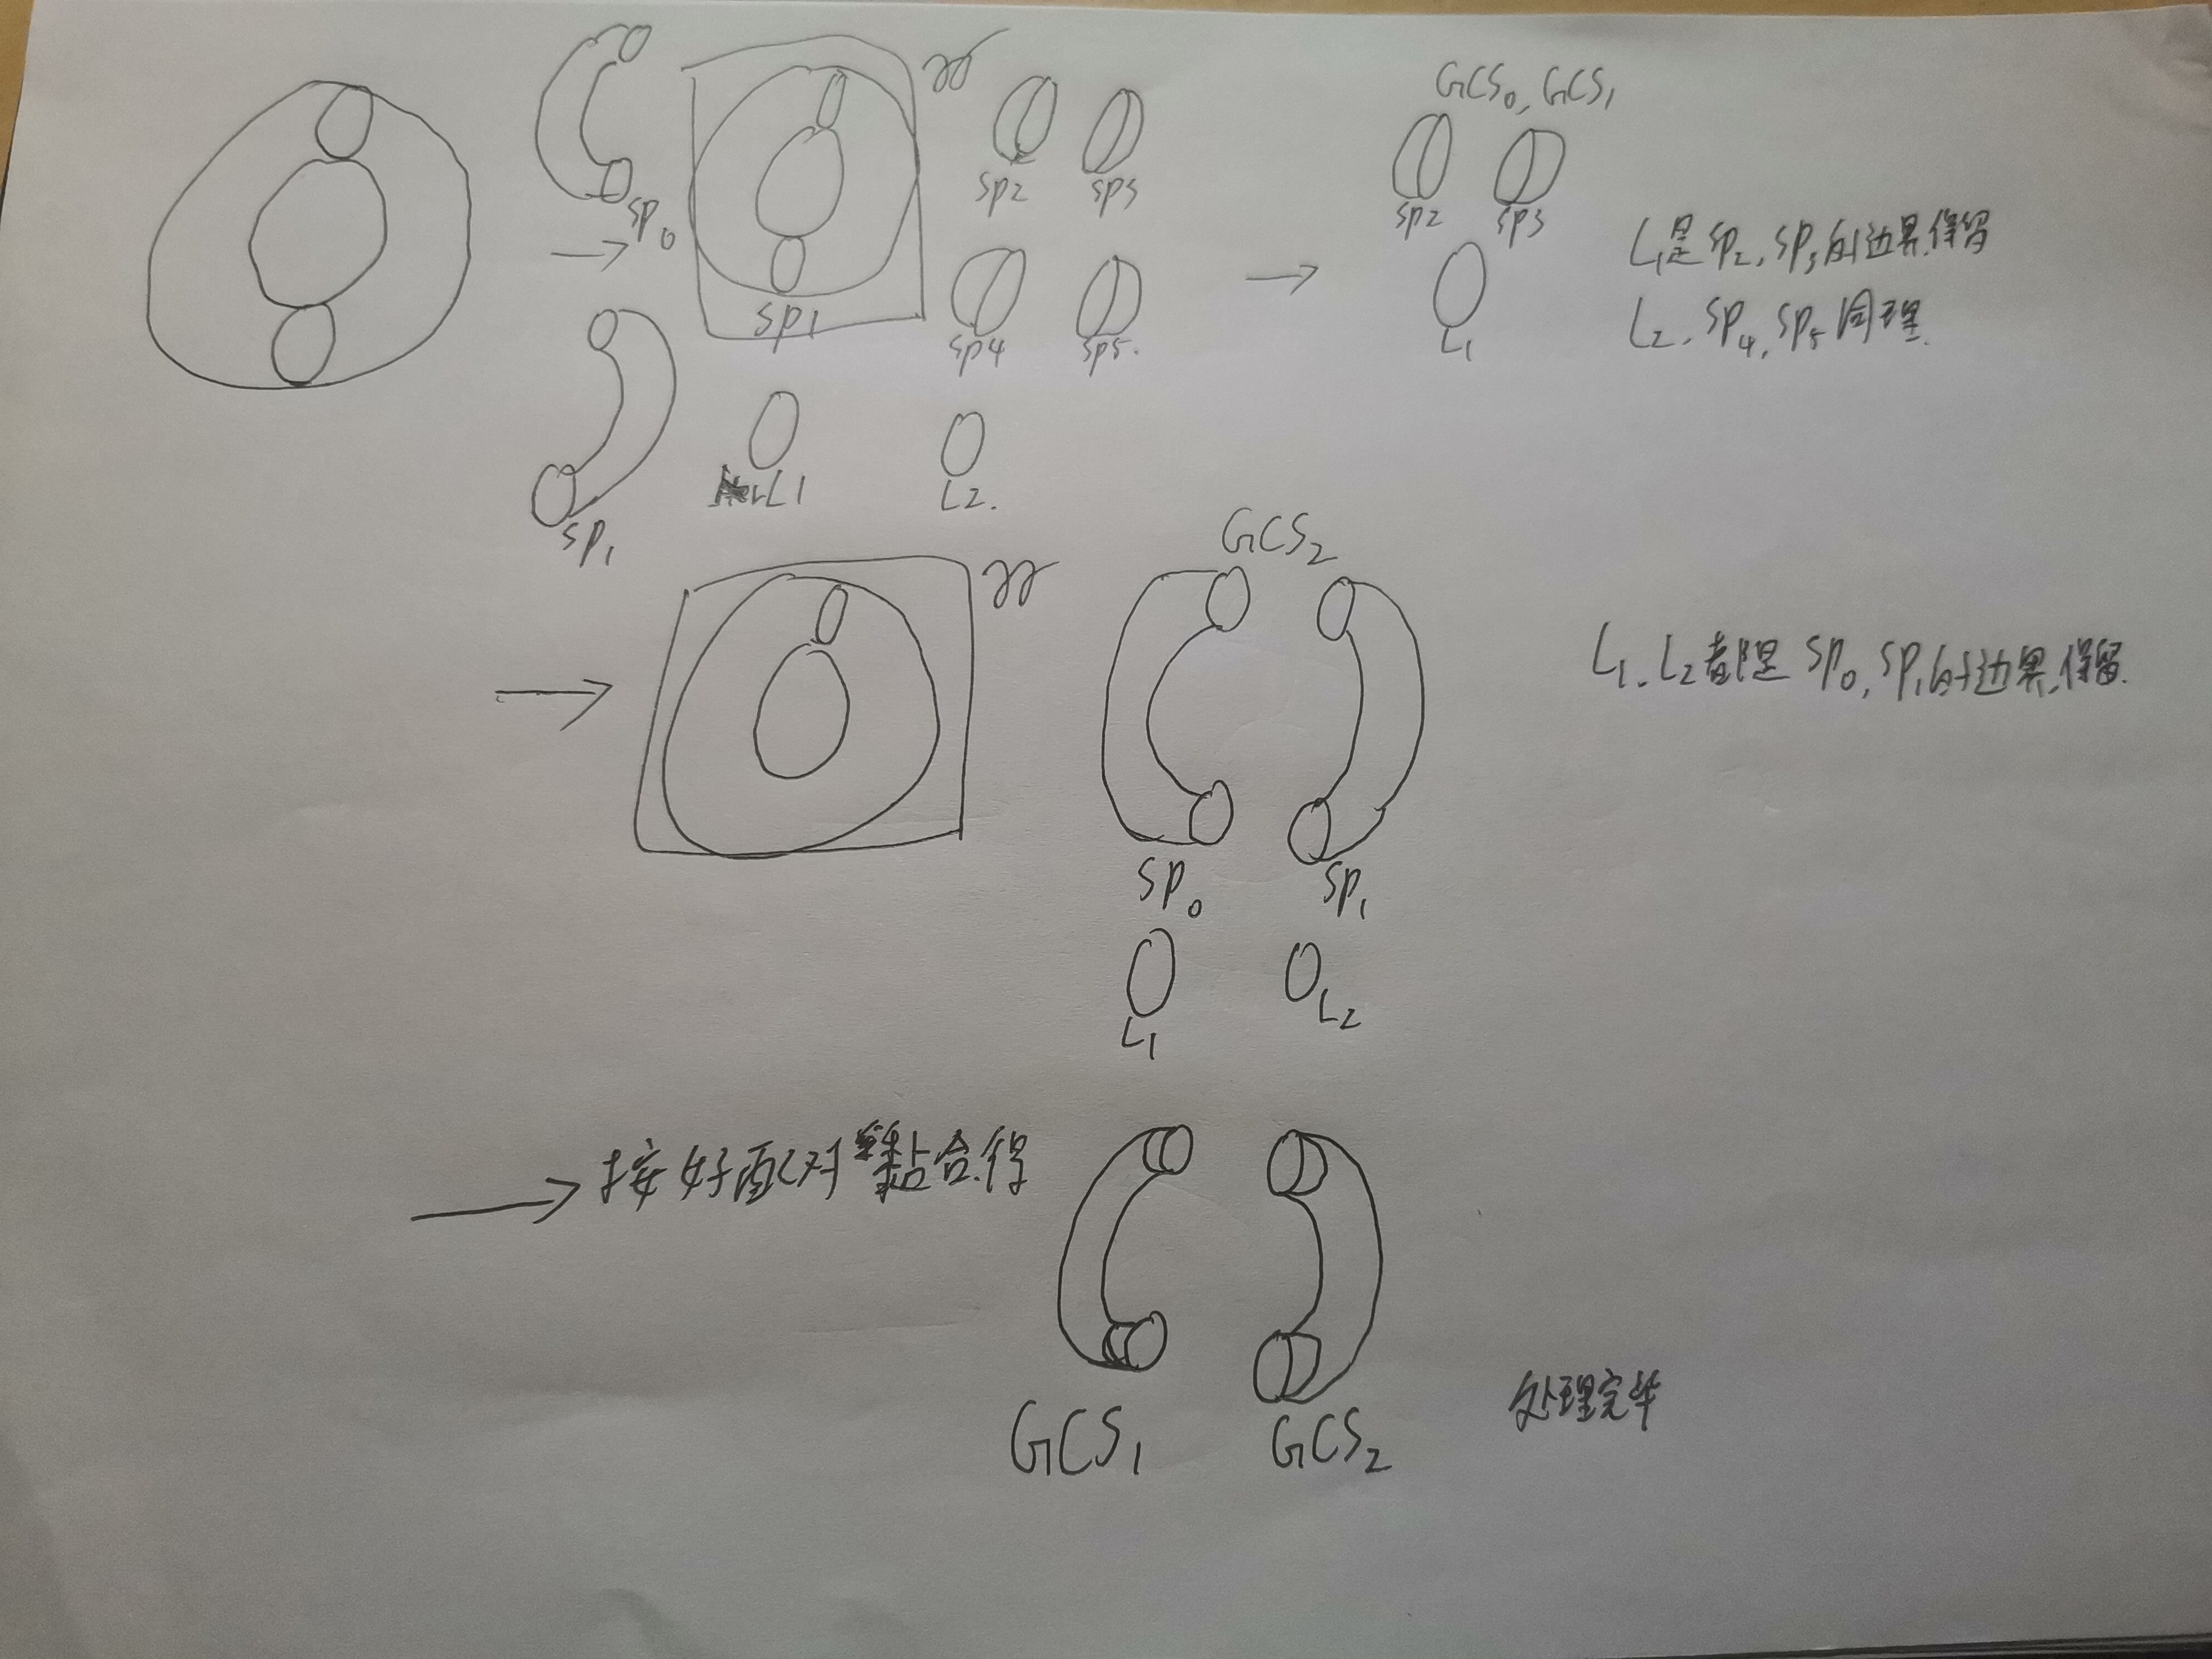
\includegraphics[width = 18cm]{fig/writing2.jpg}
% \end{figure}

% \begin{figure}
%     \caption{两条不保留的第二类交线}
%     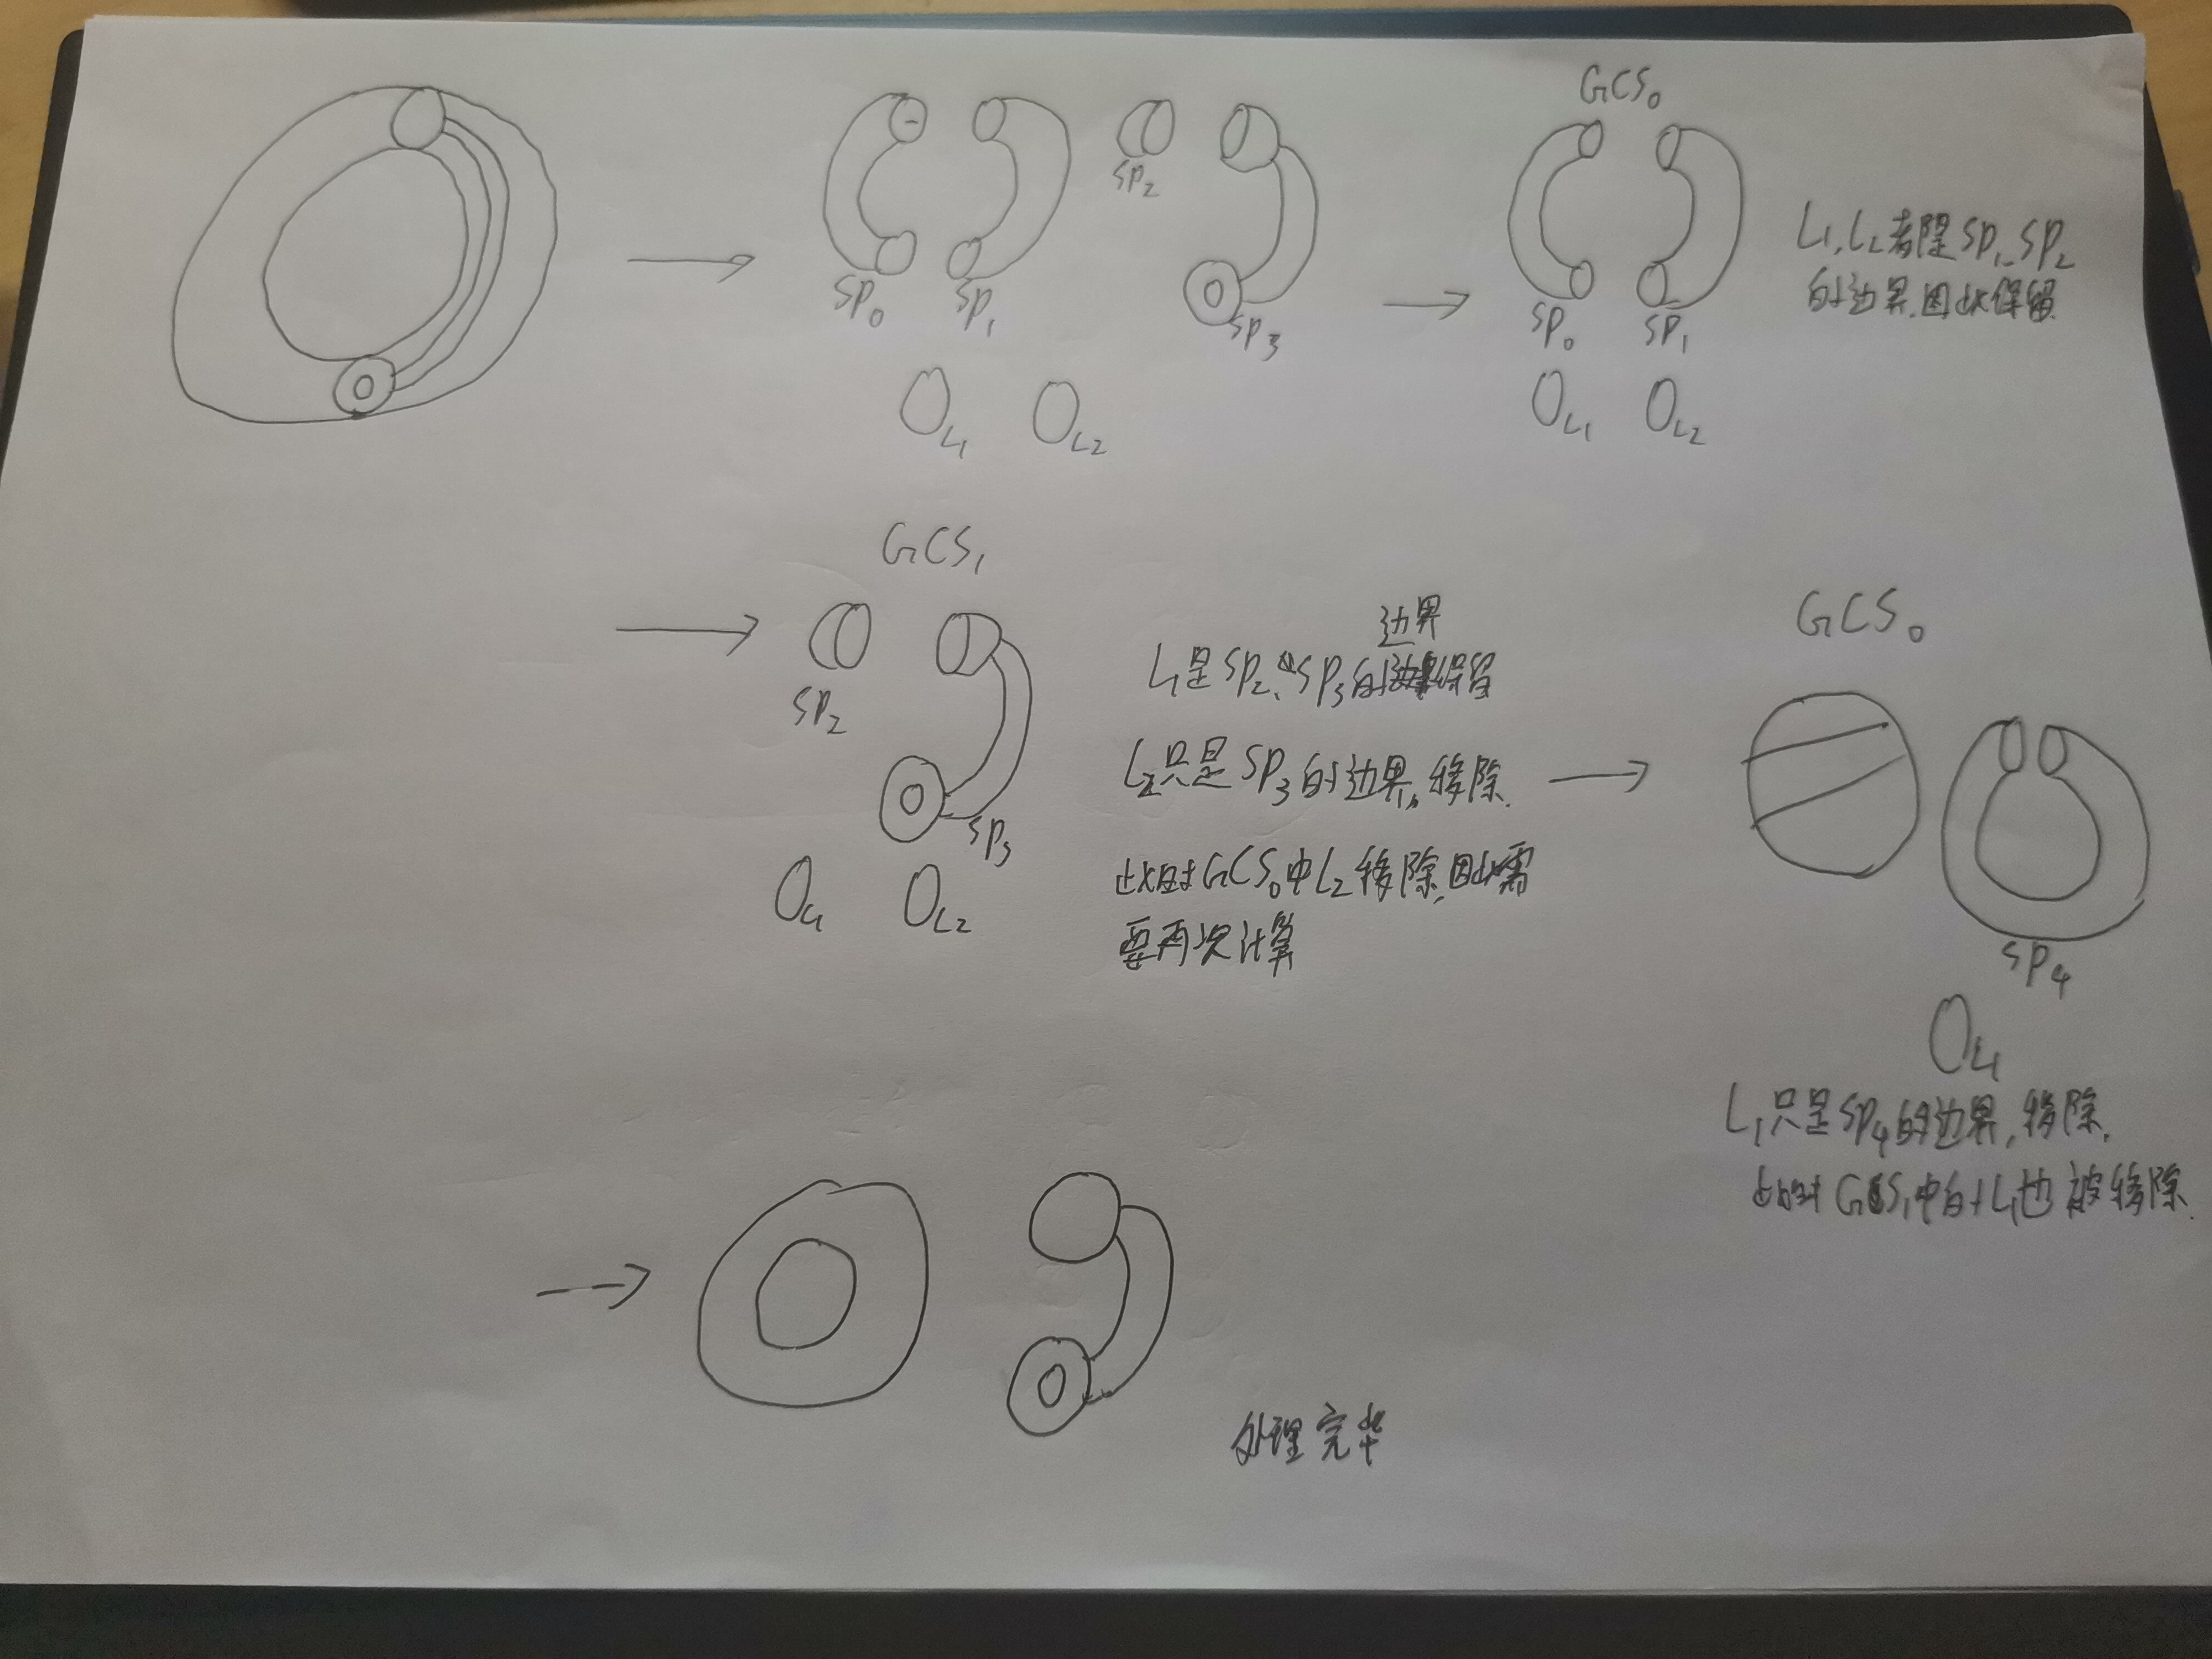
\includegraphics[width = 18cm]{fig/writing3.jpg}
% \end{figure}

% \begin{figure}
%     \caption{两条保留的第二类交线}
%     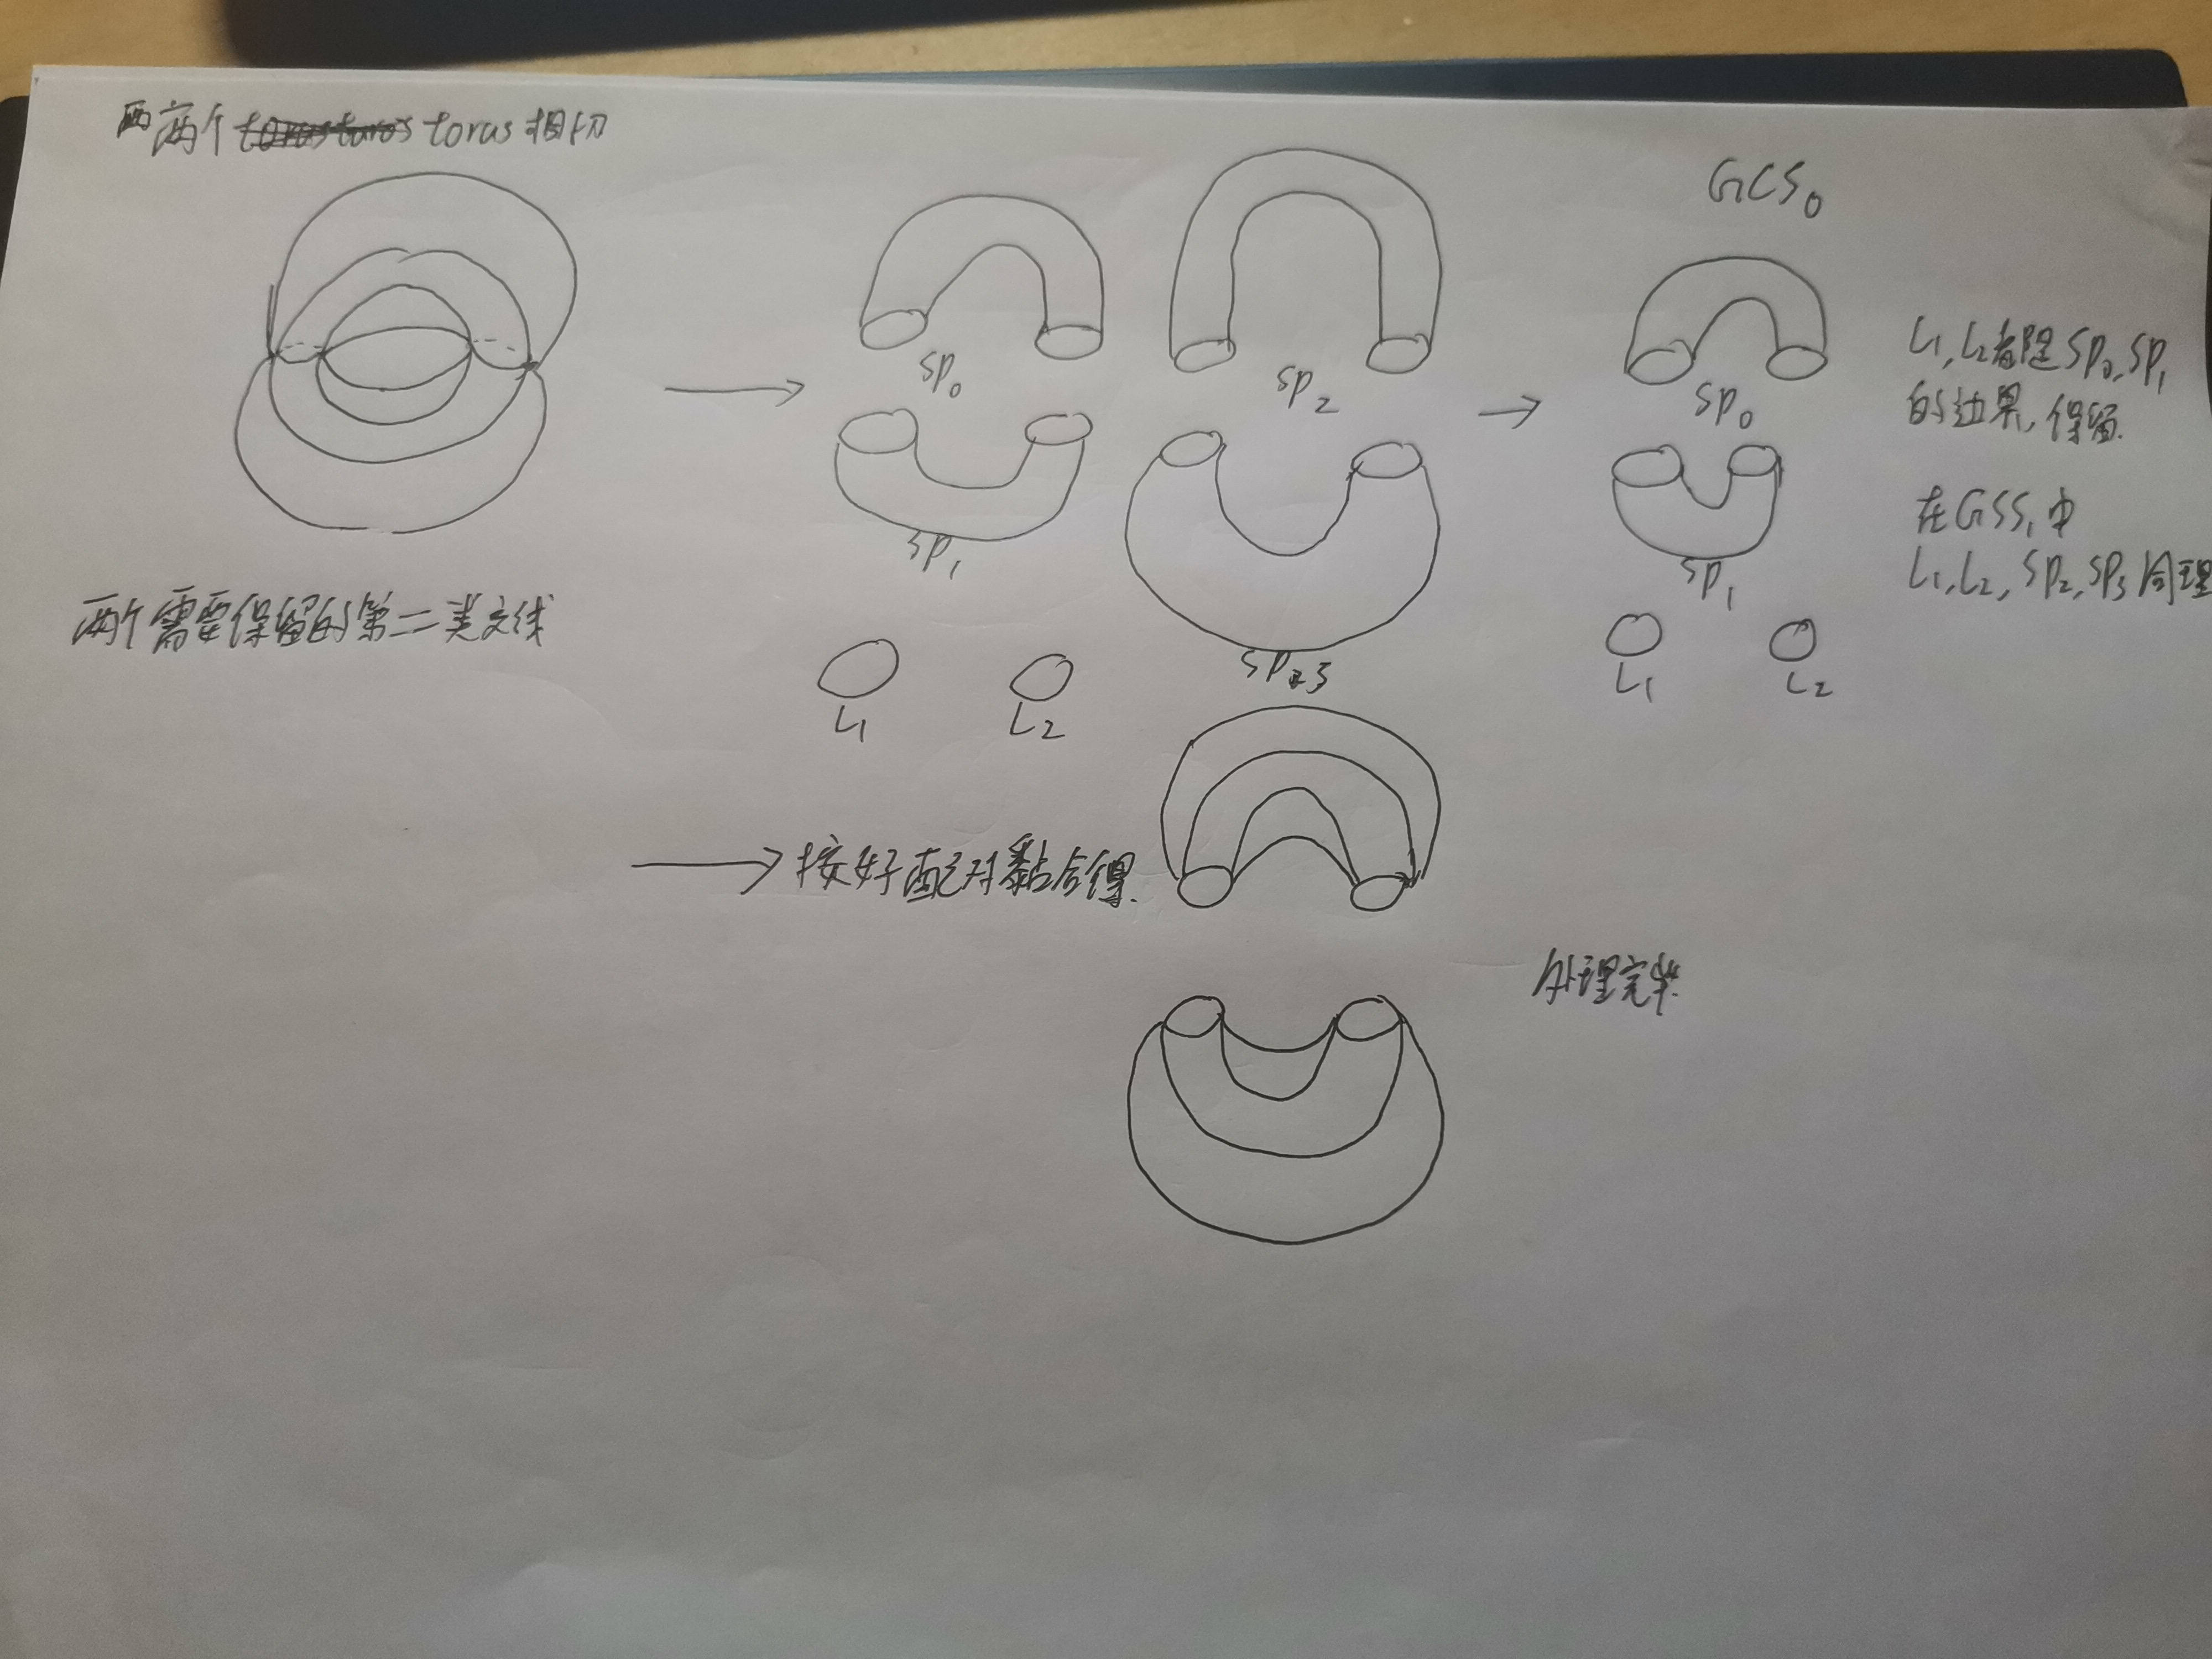
\includegraphics[width = 18cm]{fig/writing4.jpg}
% \end{figure}

% \begin{figure}
%     \caption{三条不保留的第二类交线}
%     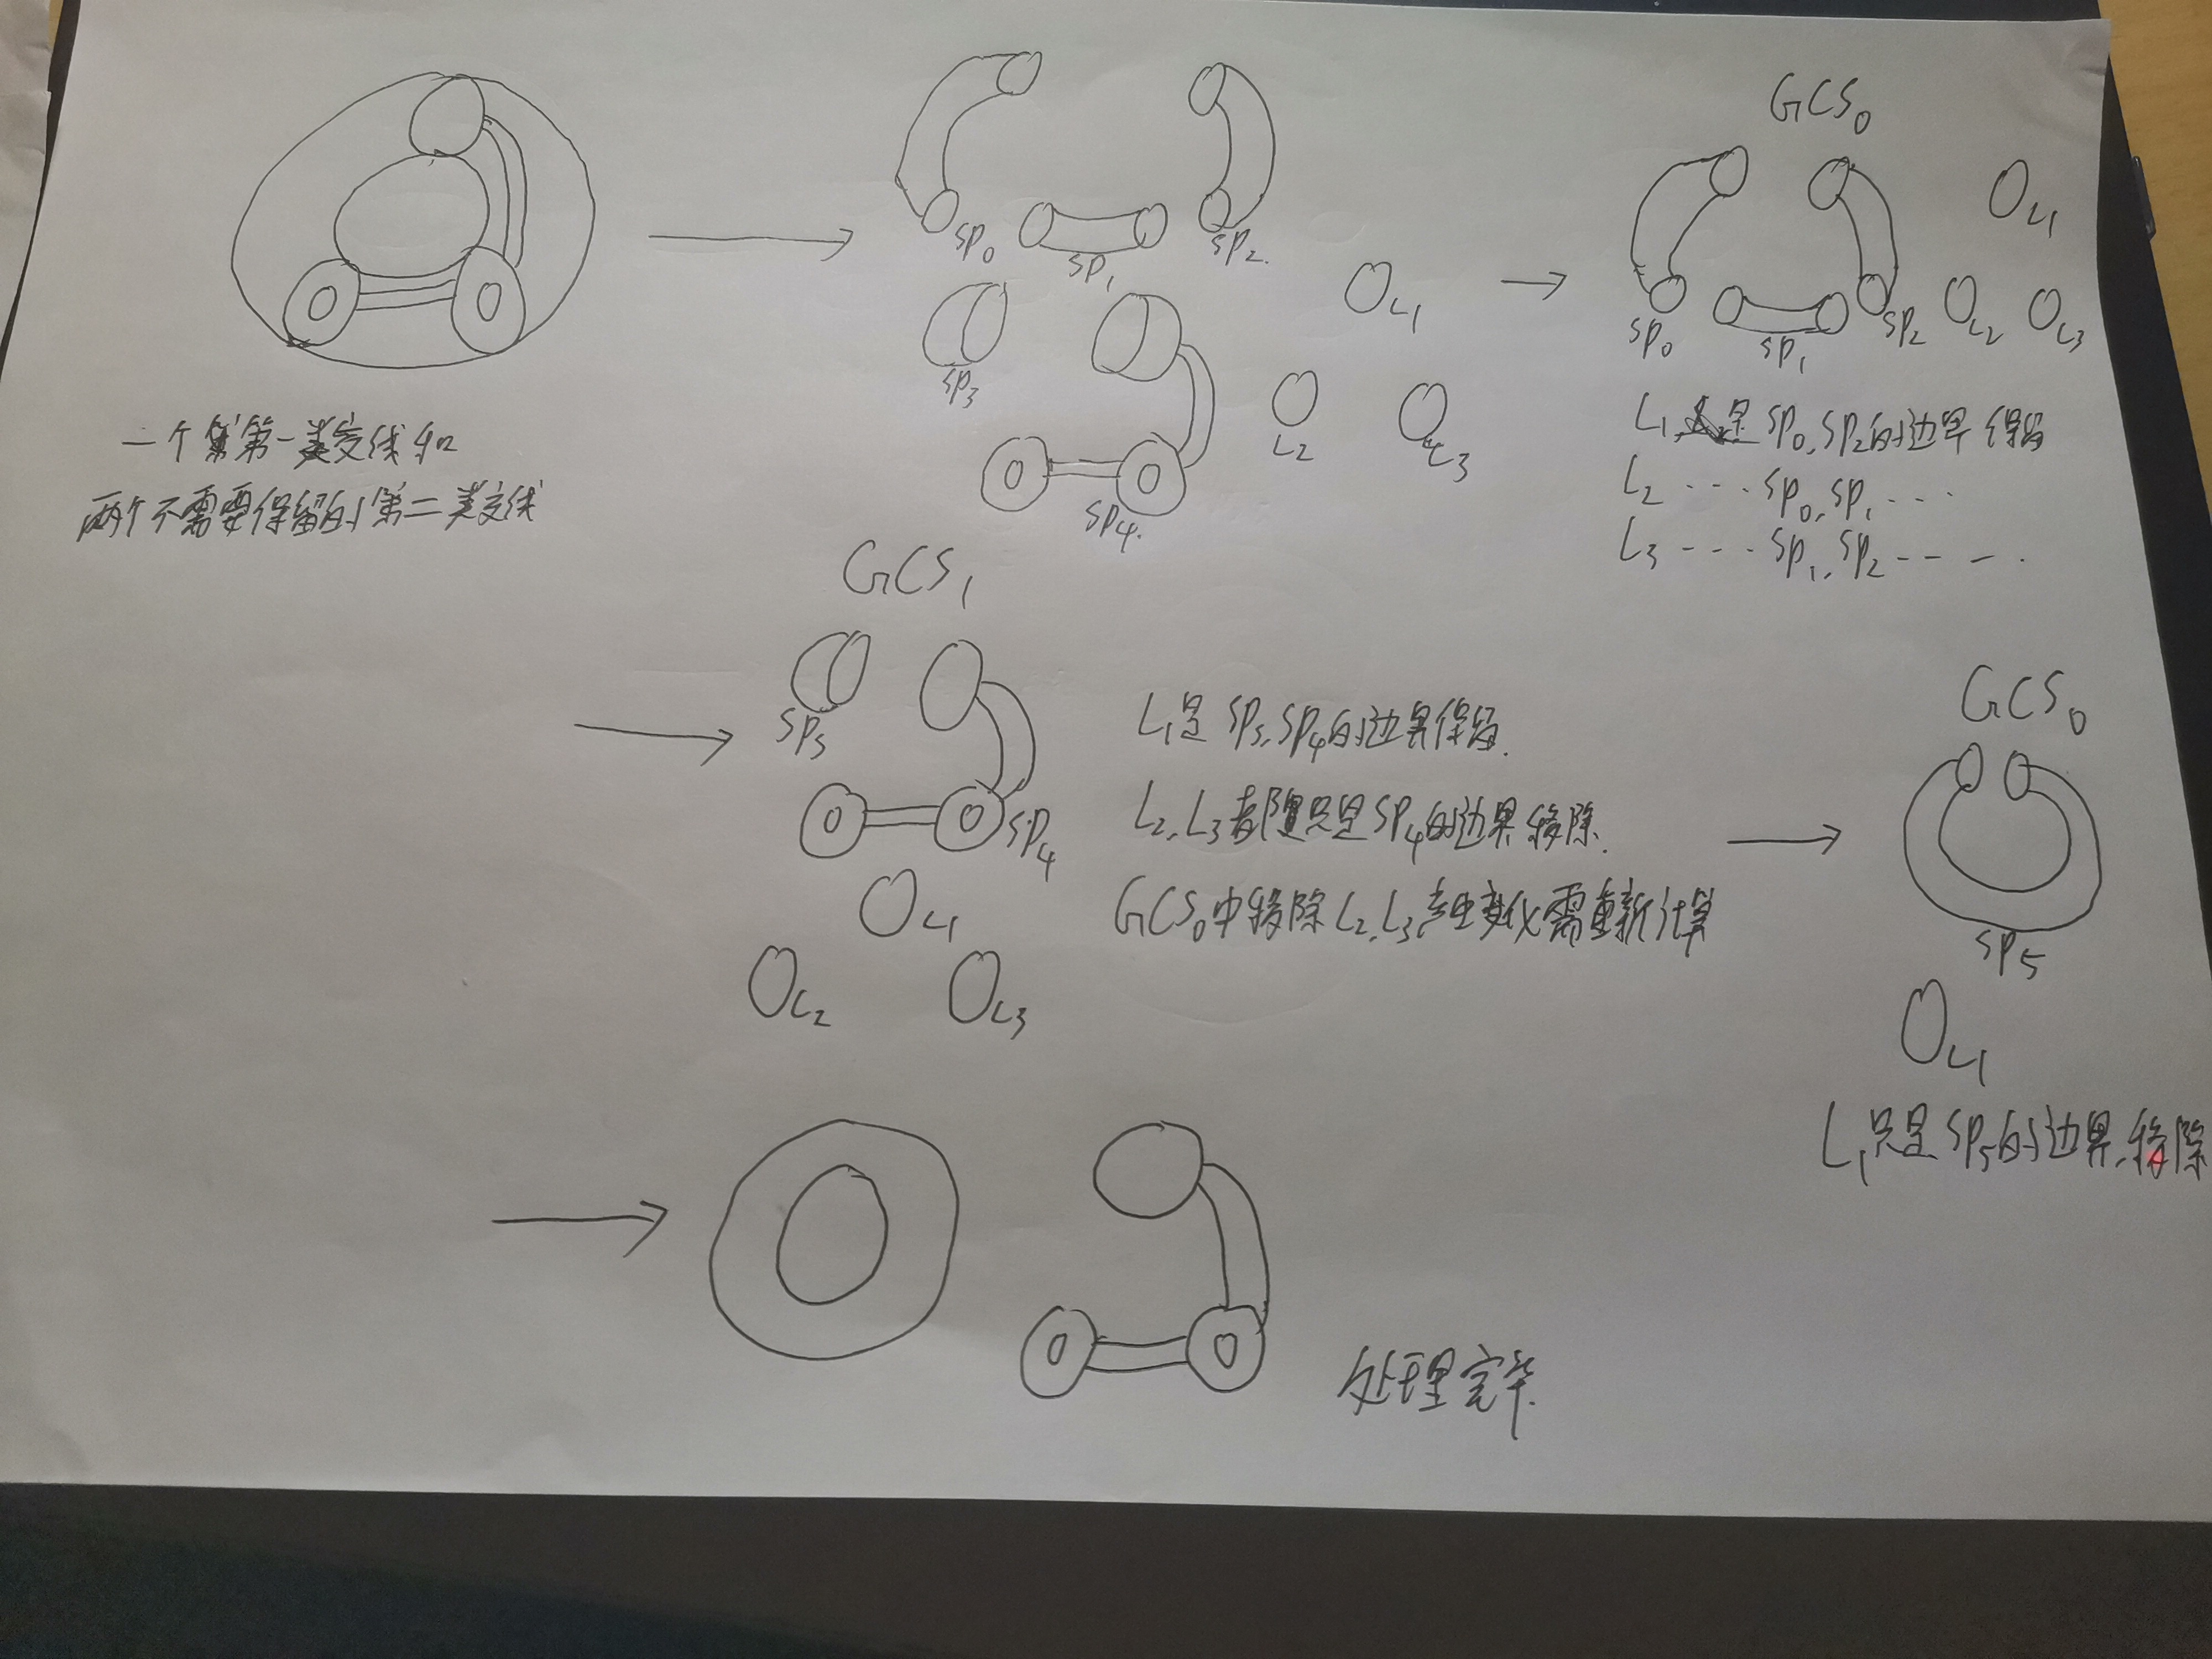
\includegraphics[width = 18cm]{fig/writing5.jpg}
% \end{figure}






    
\end{document}
